\documentclass[article,shortnames]{jss}

%% -- LaTeX packages and custom commands ------------------------------------
\usepackage{amsmath,amssymb}
\usepackage{booktabs}
\usepackage{longtable}
\usepackage{graphicx}

\newcommand{\pAm}{\{p_{Am}\}}
\newcommand{\pM}{[p_M]}
\newcommand{\EG}{[E_G]}

%% -- Article metadata ------------------------------------------------------
\author{Branimir K.~Hackenberger\\University of Osijek, SCIOM \And
        Tamara Djerdj\\University of Osijek \And
        Domagoj K.~Hackenberger\\Ru{\dj}er Bo{\v s}kovi{\'c} Institute}
\Plainauthor{Branimir K. Hackenberger, Tamara Djerdj,
             Domagoj K. Hackenberger}

\title{\pkg{BayesianDEB}: A Bayesian Framework for Dynamic Energy
       Budget Modelling in \proglang{R}}
\Plaintitle{BayesianDEB: A Bayesian Framework for Dynamic Energy Budget Modelling in R}
\Shorttitle{\pkg{BayesianDEB}: Bayesian DEB Framework in \proglang{R}}

\Abstract{
Dynamic Energy Budget (DEB) theory provides a mechanistic,
thermodynamically consistent description of how organisms acquire and
utilise energy for maintenance, growth, development, and reproduction.
Classical DEB calibration relies on deterministic optimisation, which
yields no formal uncertainty quantification and cannot naturally
accommodate prior biological knowledge or hierarchical data structures.
The \proglang{R}~package \pkg{BayesianDEB} addresses these limitations
by embedding the DEB ordinary differential equation system within a
Bayesian state-space framework, using \proglang{Stan} for Hamiltonian
Monte Carlo inference.  The package provides four pre-written
\proglang{Stan} programs covering common DEB applications: individual
growth, growth with reproduction, hierarchical multi-individual
analysis with partial pooling, and toxicokinetic-toxicodynamic (TKTD)
models for ecotoxicology.  A declarative \proglang{R} interface handles
data preparation, prior specification from biological knowledge,
observation model selection, Arrhenius temperature correction, MCMC
fitting with within-chain parallelism, convergence diagnostics,
posterior predictive checks, derived quantity estimation, and
LOO cross-validation.  We demonstrate the full workflow on simulated
\emph{Eisenia fetida} growth data, on real growth data from the
literature, and on a DEBtox analysis with EC$_{50}$/NEC
estimation.  The individual growth model is validated via
simulation-based calibration with 500~replications.  An
identifiability analysis shows that DEB rate parameters are
largely prior-dominated under single-individual growth data,
underscoring the importance of species-specific priors or
hierarchical modelling for quantitative inference.
The package is available from the SCIOM r-universe at
\url{https://sciom.r-universe.dev/BayesianDEB}; CRAN submission is
under review.
}

\Keywords{dynamic energy budget, Bayesian inference, \proglang{Stan},
  ecotoxicology, DEBtox, TKTD, hierarchical models, \proglang{R}}
\Plainkeywords{dynamic energy budget, Bayesian inference, Stan,
  ecotoxicology, DEBtox, TKTD, hierarchical models, R}

\Address{
  Branimir K.~Hackenberger\\
  Department of Biology\\
  Josip Juraj Strossmayer University of Osijek\\
  Osijek, Croatia\\
  and\\
  SCIOM d.o.o., Osijek, Croatia\\
  E-mail: \email{branimir@sciom.hr}\\
  URL: \url{https://github.com/sciom/BayesianDEB}\\[0.5em]
  %
  Tamara Djerdj\\
  Department of Biology\\
  Josip Juraj Strossmayer University of Osijek\\
  Osijek, Croatia\\[0.5em]
  %
  Domagoj K.~Hackenberger\\
  Ru{\dj}er Bo{\v s}kovi{\'c} Institute\\
  Zagreb, Croatia
}

%% -- Publication metadata (filled by JSS editors) --------------------------
\Volume{0}
\Issue{0}
\Month{April}
\Year{2026}
\Submitdate{2026-04-06}
\Acceptdate{}

\begin{document}


%% ======================================================================
\section{Introduction} \label{sec:intro}
%% ======================================================================

Dynamic Energy Budget (DEB) theory \citep{Kooijman2010} provides a
mechanistic, thermodynamically grounded framework for describing
energy acquisition, storage, and allocation across the life cycle
of an organism, and is among the most widely applied metabolic
theories in ecology and ecotoxicology.  Its core state variables
--- reserve energy~$E$, structural volume~$V$, maturity~$E_H$, and
reproduction buffer~$E_R$ --- evolve according to an ordinary
differential equation (ODE) system governed by the $\kappa$-rule:
a fraction~$\kappa$ of mobilised reserve is allocated to somatic
maintenance and growth, while the remainder funds maturity maintenance
and reproduction.

Despite its theoretical elegance, DEB calibration has traditionally
relied on deterministic least-squares or maximum-likelihood
optimisation, as implemented in \pkg{DEBtool\_M}
\citep{MarquesAmP2018} and the Add-my-Pet (AmP) online estimation
tool.  This approach yields point estimates without formal uncertainty
quantification, cannot incorporate prior biological knowledge in a
principled way, and does not naturally extend to hierarchical data
structures where multiple individuals share species-level parameters
but differ in, for example, assimilation rate.

The combination of Bayesian inference with ODE-based models is, of
course, not new \citep{GelmanBDA2013}; several authors have applied
custom MCMC to DEB \citep{JohnsonDEB2015}, and \pkg{deBInfer}
\citep{deBInfer2017} provides a general Bayesian ODE framework in
\proglang{R}.  The contribution of the present work is not a new
statistical method but a \emph{domain-specific software
system} that makes three concrete advances over existing tools:
\begin{enumerate}
  \item \emph{Unified Bayesian workflow for DEB.}  No existing tool
    combines DEB ODE models, HMC inference, observation model
    switching, Arrhenius temperature correction, convergence
    diagnostics, posterior predictive checks, derived quantity
    estimation, and LOO cross-validation in a single
    \proglang{R} interface that requires no recompilation when
    switching observation families or prior specifications.  Users of
    \pkg{DEBtool\_M} or custom \proglang{Stan} code must assemble
    this workflow manually; \pkg{BayesianDEB} provides it
    out of the box for the four most common DEB applications.
  \item \emph{Reproducible, species-specific prior system grounded
    in the AmP collection.}  The function \code{prior\_species()}
    returns priors calibrated to AmP parameter estimates
    \citep{MarquesAmP2018} for common test species, bridging the
    gap between the world's largest DEB parameter database and
    Bayesian inference.  The prior-to-posterior contraction
    diagnostic (Section~\ref{sec:identifiability}) quantifies
    how much the data inform each parameter beyond the prior ---
    a transparency that deterministic calibration cannot offer.
  \item \emph{Inference validation for the individual growth model.}
    Simulation-based calibration
    (Section~\ref{sec:sbc}) with 500~replications and formal
    $\chi^2$ uniformity tests demonstrates, conditional on MCMC
    convergence, that the individual growth model is well-calibrated.
    Preliminary SBC evidence for the hierarchical model is also
    provided.  To our knowledge, this level of algorithmic
    validation has not been reported for any DEB calibration tool.
\end{enumerate}
Together, these advances lower the barrier to rigorous Bayesian DEB
modelling from expert \proglang{Stan} programming to a declarative
\proglang{R} call, while making identifiability limitations and
prior sensitivity explicit rather than hidden.

\emph{Important caveat.}  As our identifiability analysis
(Section~\ref{sec:identifiability}) demonstrates, growth-only data
from a single individual cannot resolve the individual contributions
of the DEB rate parameters $\pAm$, $\pM$, $v$; posteriors for these
parameters are substantially shaped by the prior even with dense
time series.  Species-specific informative priors or hierarchical
data structures are essential for quantitative inference.
\pkg{BayesianDEB} makes this limitation \emph{visible} through
contraction diagnostics and prior sensitivity tools, whereas
deterministic calibration tools obscure it behind point estimates.

The \pkg{BayesianDEB} package wraps four \proglang{Stan}
\citep{CarpenterStan2017} programs with a declarative \proglang{R}
interface.  The package implements:
\begin{itemize}
  \item Individual-level growth (2-state: $E$, $V$).
  \item Growth with reproduction (3-state: $E$, $V$, $E_R$).
  \item Hierarchical multi-individual growth with partial pooling on
    $\pAm$ via a non-centred parameterisation
    \citep{BetancourtHierarchical2015}.
  \item DEBtox toxicokinetic-toxicodynamic (TKTD) models following
    \citet{JagerDEBtox2006}, with analytical EC$_{50}$ and NEC
    computation.
\end{itemize}

All models support switchable observation families (Gaussian,
log-normal, Student-$t$ for growth; negative binomial or Poisson for
reproduction), Arrhenius temperature correction, within-chain
parallelism via \proglang{Stan}'s \code{reduce\_sum}, and a suite of
diagnostic and visualisation tools.

This paper describes \pkg{BayesianDEB} version~0.1.2.  The package is
available from the SCIOM r-universe at
\url{https://sciom.r-universe.dev/BayesianDEB} (CRAN submission
under review) and from GitHub
at \url{https://github.com/sciom/BayesianDEB}.


%% ======================================================================
\section{DEB theory and model formulation} \label{sec:theory}
%% ======================================================================

We summarise the DEB equations implemented in \pkg{BayesianDEB} and
discuss modelling choices; for a full treatment see
\citet{Kooijman2010}.  The standard DEB model is one of several
metabolic frameworks; alternatives include the ``standard'' and
``abj'' typified models in the AmP collection \citep{MarquesAmP2018},
net-production models, and various simplified formulations
\citep{JagerZimmer2012}.  \pkg{BayesianDEB} implements the standard
($\kappa$-rule) formulation, which is the most widely used and has the
largest empirical parameter base via AmP.

\subsection{Standard DEB: growth} \label{sec:growth}

The two core state variables are reserve energy $E$~(J) and structural
volume $V$~(cm$^3$), with structural length $L = V^{1/3}$.  Under
constant food availability characterised by the scaled functional
response $f \in [0, 1]$, the energy fluxes are:
\begin{align}
  \dot{p}_A &= f \, \pAm \, L^2,  \label{eq:pA} \\
  \dot{p}_C &= \frac{E \, v \, L}{E + \EG \, V},  \label{eq:pC} \\
  \dot{p}_M &= \pM \, V,  \label{eq:pM}
\end{align}
where $\pAm$ is the surface-area-specific maximum assimilation rate
(J\,d$^{-1}$\,cm$^{-2}$), $v$ is the energy conductance
(cm\,d$^{-1}$), $\EG$ is the specific cost of structure
(J\,cm$^{-3}$), and $\pM$ is the volume-specific somatic maintenance
rate (J\,d$^{-1}$\,cm$^{-3}$).  The state equations are:
\begin{align}
  \frac{dE}{dt} &= \dot{p}_A - \dot{p}_C,  \label{eq:dE} \\
  \frac{dV}{dt} &= \frac{\kappa \, \dot{p}_C - \dot{p}_M}{\EG},
    \label{eq:dV}
\end{align}
where $\kappa$ is the allocation fraction to soma.  At steady state
($dV/dt = 0$, $dE/dt = 0$), the ultimate structural length is
$L_\infty = f \, \kappa \, \pAm / \pM$.

\paragraph{Edge cases.}
When $\kappa \dot{p}_C < \dot{p}_M$ (starvation), growth ceases and
the organism draws on structure for maintenance; in our implementation
$dV/dt$ is clamped to zero to prevent negative structural volume.
When $\kappa \to 0$, nearly all mobilised energy goes to reproduction
and growth is negligible; when $\kappa \to 1$, reproduction ceases.
The Beta prior on $\kappa$ (default $\mathrm{Beta}(2,2)$) regularises
the posterior away from these boundary cases.

\paragraph{ODE stiffness and solver choice.}
DEB systems are mildly stiff due to the time-scale separation between
fast reserve dynamics and slow structural growth.  The mobilisation
flux $\dot{p}_C = EvL / (E + \EG V)$ creates stiffness when $E \gg
\EG V$ (near steady-state reserve).  We use the BDF (backward
differentiation formula) solver \code{ode\_bdf\_tol} with tolerances
$10^{-6}$, which is standard for mildly stiff biological ODE systems.
The explicit Runge-Kutta solver (\code{ode\_rk45}) was also tested:
it produced identical trajectories for well-conditioned parameter
regions but required approximately $2\times$ more function evaluations
and occasionally failed for extreme parameter combinations during MCMC
warmup.  The BDF solver was therefore chosen as the safer default.

\subsection{Growth with reproduction} \label{sec:repro}

For post-pubertal organisms ($E_H \geq E_H^p$), adding the
reproduction buffer $E_R$~(J) yields a 3-state model:
\begin{equation}
  \frac{dE_R}{dt} = (1 - \kappa) \, \dot{p}_C - k_J \, E_H^p,
    \label{eq:dR}
\end{equation}
where $k_J$ is the maturity maintenance rate coefficient and $E_H^p$
is maturity at puberty (treated as a known constant, not a state
variable, since the model describes post-pubertal growth only).  Offspring counts over an interval
$[t_s, t_e]$ are modelled as
$R \sim \mathrm{NegBin}_2(\mu = k_R \, \Delta E_R,\, \phi)$,
where $\Delta E_R = E_R(t_e) - E_R(t_s)$, $k_R$ is the buffer-to-offspring
conversion rate (offspring\,J$^{-1}$), $\mu$ is the expected count, and
$\phi > 0$ is the overdispersion parameter.  This uses \proglang{Stan}'s
\code{neg\_binomial\_2} parametrisation, where $\mathrm{E}[R] = \mu$
and $\mathrm{Var}[R] = \mu + \mu^2/\phi$; as
$\phi \to \infty$ the distribution converges to
$\mathrm{Poisson}(\mu)$.

\subsection{DEBtox: toxicokinetic-toxicodynamic extension}
\label{sec:debtox}

The DEBtox framework \citep{JagerDEBtox2006, JagerZimmer2012} adds a
scaled internal damage variable~$D_w$:
\begin{equation}
  \frac{dD_w}{dt} = k_d \bigl(\max(C_w - z_w, 0) - D_w\bigr),
    \label{eq:Dw}
\end{equation}
where $k_d$ is the damage recovery rate, $C_w$ is the external
concentration, and $z_w$ is the no-effect concentration (NEC).  The
damage causes a stress factor $s = b_w \, D_w$ that reduces
assimilation: $\dot{p}_A \leftarrow \dot{p}_A \cdot \max(1 - s, 0)$.
At steady state, $D_w = C_w - z_w$ for $C_w > z_w$, so the
EC$_{50}$ for 50\% assimilation reduction is:
\begin{equation}
  \mathrm{EC}_{50} = z_w + \frac{0.5}{b_w}.
    \label{eq:EC50}
\end{equation}

\subsection{Arrhenius temperature correction} \label{sec:arrhenius}

All rate parameters scale with temperature by the factor
$c_T = \exp(T_A / T_{\mathrm{ref}} - T_A / T)$
\citep[Eq.~1.2]{Kooijman2010}, where $T_A$ is the Arrhenius
temperature (species-specific, typically 6000--12\,000~K).  In
\pkg{BayesianDEB}, the correction is applied inside the
\proglang{Stan} ODE to $\pAm$, $\pM$, $v$, $k_J$, and $k_d$;
the estimated parameters correspond to the reference temperature
$T_{\mathrm{ref}}$.

\subsection{Hierarchical structure} \label{sec:hierarchical}

When data from multiple individuals are available, a lognormal random
effect on $\pAm$ is introduced via the non-centred parameterisation
\citep{BetancourtHierarchical2015}:
\begin{equation}
  \log \pAm_j = \mu_{\log \pAm} + \sigma_{\log \pAm} \cdot z_j,
  \qquad z_j \sim \mathcal{N}(0, 1).
    \label{eq:hier}
\end{equation}
The shared parameters $\pM$, $\kappa$, $v$, $\EG$ are estimated from
all individuals jointly (partial pooling).

\paragraph{Why random effects on $\pAm$ only?}
In DEB theory, $\pAm$ is the parameter most strongly linked to
individual phenotypic variation: it determines food uptake capacity and
scales with structural surface area, which varies among individuals
due to differences in condition, microhabitat, and genotype.  The
energy conductance~$v$, maintenance~$\pM$, and costs~$\EG$ are
typically more conserved within a species \citep{Kooijman2010,
MarquesAmP2018}.  Placing random effects on all parameters
simultaneously would create a high-dimensional, poorly identified
model for typical DEB dataset sizes (5--30 individuals with 5--15
time points each).  The single-random-effect design is a deliberate
parsimony choice; extension to multivariate random effects on
$(\pAm, \kappa)$ or $(\pAm, L_0)$ is planned for a future version
once identifiability under realistic sample sizes has been formally
assessed.


%% ======================================================================
\section{Bayesian state-space formulation} \label{sec:statespace}
%% ======================================================================

We now formalise the statistical model.  Let $\mathbf{x}(t) = (E(t),
V(t))^\top$ (or $(E, V, E_R)^\top$, $(E, V, E_R, D_w)^\top$ for the
extended models) denote the latent DEB state, and let
$\boldsymbol{\theta}$ collect the DEB parameters.

\subsection{Process model}

The latent state evolves deterministically according to the ODE:
\begin{equation}
  \frac{d\mathbf{x}}{dt} = \mathbf{f}(\mathbf{x}, \boldsymbol{\theta},
  f, C_w), \qquad \mathbf{x}(0) = \mathbf{x}_0(\boldsymbol{\theta}),
  \label{eq:ode_general}
\end{equation}
where $\mathbf{f}$ is defined by
Equations~\eqref{eq:dE}--\eqref{eq:dV} (growth),
\eqref{eq:dR} (reproduction), or \eqref{eq:Dw} (DEBtox), and
$\mathbf{x}_0$ depends on initial conditions $(E_0, L_0)$.

\subsection{Observation model}

Given the ODE solution $\hat{L}_i = [\mathbf{x}(t_i)]_V^{1/3}$,
the growth observations are conditionally independent:
\begin{equation}
  L_i^{\mathrm{obs}} \mid \hat{L}_i, \sigma_L \;\sim\;
  \begin{cases}
    \mathcal{N}(\hat{L}_i,\, \sigma_L) & \text{(Gaussian)}, \\
    \mathrm{LogNormal}(\log\hat{L}_i,\, \sigma_L) & \text{(log-normal)}, \\
    t_\nu(\hat{L}_i,\, \sigma_L) & \text{(Student-}t\text{)}.
  \end{cases}
  \label{eq:obs_L}
\end{equation}
For reproduction, interval offspring counts use \proglang{Stan}'s
mean-overdispersion parametrisation
(\code{neg\_binomial\_2}):
\begin{equation}
  R_k \mid \mu_k, \phi \;\sim\;
  \mathrm{NegBin}_2(\mu_k,\, \phi)
  \quad\text{or}\quad
  \mathrm{Poisson}(\mu_k),
  \qquad \mu_k = k_R \, \Delta E_{R,k},
  \label{eq:obs_R}
\end{equation}
where $\mathrm{E}[R_k] = \mu_k$ and $\mathrm{Var}[R_k] = \mu_k +
\mu_k^2 / \phi$.

\subsection{Prior model}

The full prior factorises as:
\begin{equation}
  p(\boldsymbol{\theta}) = p(\pAm) \, p(\pM) \, p(\kappa) \, p(v) \,
  p(\EG) \, p(E_0) \, p(L_0) \, p(\sigma_L) \, [\text{model-specific}].
  \label{eq:prior}
\end{equation}
Default prior families are: $\pAm, \pM, v, \EG \sim
\mathrm{LogNormal}$; $\kappa \sim \mathrm{Beta}$; $\sigma_L \sim
\mathrm{HalfNormal}$ \citep[following the recommendations
of][]{GelmanPriorVariance2006}.  Hyperparameters are calibrated
against the AmP collection ranges \citep{MarquesAmP2018} and passed
to \proglang{Stan} as data, so that changing priors does not require
recompilation.

\paragraph{Prior calibration rationale.}
Table~\ref{tab:priors} shows the \emph{generic} default
hyperparameters (\code{prior\_default()}) and their implied 95\%
prior mass ranges.  These are deliberately wide ($\sigma = 1.0$)
to accommodate any species; they are \emph{not} suitable for
quantitative inference without tightening (see
Section~\ref{sec:prior_sens}).

For common test species, the function \code{prior\_species()} returns
priors calibrated to the AmP collection \citep{MarquesAmP2018},
with $\sigma = 0.3$ for well-characterised parameters:
\begin{CodeChunk}
\begin{CodeInput}
R> prior_species("Eisenia_fetida")
R> prior_species("Daphnia_magna", type = "debtox")
\end{CodeInput}
\end{CodeChunk}
\noindent
Built-in species include \emph{Eisenia fetida}, \emph{E.~andrei},
\emph{Folsomia candida}, \emph{Daphnia magna}, and
\emph{Lumbricus rubellus}.  Users working with other species should
construct custom priors from the relevant AmP entry.  We recommend
always conducting a prior sensitivity analysis
(Section~\ref{sec:prior_sens}).

\begin{table}[t!]
\centering
\caption{Default prior specifications and implied ranges, compared
  with AmP empirical ranges for earthworms and springtails.}
\label{tab:priors}
\begin{tabular}{llrrl}
\toprule
Parameter & Prior family & $\mu$ / $a$ & $\sigma$ / $b$ &
  95\% prior range \\
\midrule
$\pAm$    & LogNormal & 1.0  & 1.0  & 0.4--20 \\
$\pM$     & LogNormal & $-$1.0 & 1.0 & 0.04--2 \\
$\kappa$  & Beta      & 2    & 2    & 0.09--0.91 \\
$v$       & LogNormal & $-$1.5 & 1.0 & 0.02--1 \\
$\EG$     & LogNormal & 6.0  & 1.0  & 100--3000 \\
$\sigma_L$ & HalfNormal & 0 & 0.1 & 0--0.2 \\
\bottomrule
\end{tabular}
\end{table}

\subsection{Joint posterior}

The posterior is:
\begin{equation}
  p(\boldsymbol{\theta} \mid \mathbf{y}) \;\propto\;
  p(\boldsymbol{\theta}) \prod_{i=1}^{N_L}
  p(L_i^{\mathrm{obs}} \mid \hat{L}_i(\boldsymbol{\theta}), \sigma_L)
  \prod_{k=1}^{N_R}
  p(R_k \mid \Delta E_{R,k}(\boldsymbol{\theta}), k_R, \phi),
  \label{eq:posterior}
\end{equation}
sampled via the No-U-Turn Sampler \citep[NUTS;][]{HoffmanNUTS2014}
with a stiff BDF ODE solver evaluated at each leapfrog step.

\subsection{Hierarchical extension}

For $J$ individuals with individual random effects on $\pAm$, the
hierarchical model adds population-level hyperparameters
$\mu_{\log \pAm}$ and $\sigma_{\log \pAm}$:
\begin{equation}
  \log \pAm_j \mid \mu, \sigma \;\sim\; \mathcal{N}(\mu, \sigma),
  \qquad j = 1, \ldots, J.
  \label{eq:hier_formal}
\end{equation}
The non-centred reparameterisation $\log \pAm_j = \mu + \sigma \cdot
z_j$, $z_j \sim \mathcal{N}(0,1)$ avoids the pathological funnel
geometry \citep{BetancourtHierarchical2015}.


%% ======================================================================
\section[BayesianDEB: Software design]{%
  \pkg{BayesianDEB}: Software design} \label{sec:design}
%% ======================================================================

\subsection{Architecture} \label{sec:architecture}

The package consists of three layers:
\begin{description}
  \item[\proglang{Stan} models.] Four pre-written \code{.stan} programs
    in \code{inst/stan/}, implementing the DEB ODE system with
    the variadic \code{ode\_bdf\_tol} solver (BDF, tolerances
    $10^{-6}$).  The hierarchical and DEBtox models use
    \code{reduce\_sum} for within-chain parallelism.  Observation model
    switching (Gaussian / log-normal / Student-$t$ for growth; negative
    binomial / Poisson for reproduction) is controlled by integer flags
    in the \proglang{Stan} data block, avoiding recompilation when
    changing observation families or prior hyperparameters.
    Structural model changes (e.g., adding state variables or
    reparametrising in terms of derived quantities) require
    modifying the underlying \proglang{Stan} programs.
  \item[\proglang{R} interface.] Exported functions for data
    preparation (\code{bdeb\_data}), model specification
    (\code{bdeb\_model}), MCMC fitting (\code{bdeb\_fit}), diagnostics
    (\code{bdeb\_diagnose}), posterior predictive checks
    (\code{bdeb\_ppc}), derived quantities (\code{bdeb\_derived}), LOO
    cross-validation (\code{bdeb\_loo}), prior predictive simulation
    (\code{bdeb\_prior\_predictive}), reproducibility reporting
    (\code{bdeb\_session\_info}), and standalone ODE simulators
    (\code{deb\_simulate}, \code{debtox\_simulate}).  All
    functions use S3 classes (\code{bdeb\_data}, \code{bdeb\_model},
    \code{bdeb\_fit}) with \code{print}, \code{plot}, \code{summary},
    \code{coef}, and \code{predict} methods.
  \item[Prior system.] A family of \code{prior\_*()} constructors
    (\code{prior\_lognormal}, \code{prior\_beta},
    \code{prior\_halfnormal}, \code{prior\_halfcauchy},
    \code{prior\_exponential}, \code{prior\_normal}) that encode
    distribution choices as lightweight S3 objects.  Weakly informative
    defaults calibrated against the AmP collection
    \citep{MarquesAmP2018} are provided via \code{prior\_default()}.
\end{description}

\subsection{Workflow} \label{sec:workflow}

The recommended workflow follows the iterative Bayesian modelling cycle
of \citet[Ch.~6]{GelmanBDA2013}:
\begin{enumerate}
  \item Prepare and validate data with \code{bdeb\_data()}.
  \item Specify model, priors, and observation family with
    \code{bdeb\_model()}.
  \item Fit via MCMC with \code{bdeb\_fit()}.
  \item Check convergence with \code{bdeb\_diagnose()}
    ($\hat{R}$, ESS, divergences; \citealp{VehtariRhat2021}).
  \item Perform posterior predictive checks with \code{bdeb\_ppc()}.
  \item Compute derived quantities with \code{bdeb\_derived()}.
  \item Compare models via \code{bdeb\_loo()}
    \citep{VehtariLOO2017}.
  \item Iterate: revise priors or model structure as needed.
\end{enumerate}

\subsection{Observation models} \label{sec:obs}

The observation model is selected via constructor functions passed to
the \code{observation} argument of \code{bdeb\_model()}:
\begin{CodeChunk}
\begin{CodeInput}
R> mod <- bdeb_model(dat, type = "individual",
+    observation = list(growth = obs_student_t(nu = 5)))
\end{CodeInput}
\end{CodeChunk}
The choice is encoded as an integer flag in the \proglang{Stan} data
block (\code{obs\_growth = 1/2/3}, \code{obs\_repro = 1/2}) and
dispatched via conditional blocks in the model and generated quantities
sections.  This avoids recompilation when switching families.

\subsection{Temperature correction} \label{sec:temp_impl}

If a \code{temperature} list is supplied to \code{bdeb\_model()}, the
Arrhenius correction factor $c_T$ is computed in the \proglang{Stan}
\code{transformed data} block and applied to all rate parameters inside
the ODE.  The posterior gives estimates at $T_{\mathrm{ref}}$, making
results comparable across experiments at different temperatures.

\subsection{Within-chain parallelism} \label{sec:threading}

The hierarchical and DEBtox models distribute per-individual (or
per-group) ODE solves across threads via \proglang{Stan}'s
\code{reduce\_sum}.  The \code{threads\_per\_chain} argument in
\code{bdeb\_fit()} controls this:
\begin{CodeChunk}
\begin{CodeInput}
R> fit <- bdeb_fit(mod, chains = 4, threads_per_chain = 4)
\end{CodeInput}
\end{CodeChunk}


%% ======================================================================
\section{Illustrations} \label{sec:illustrations}
%% ======================================================================

We illustrate three of the four model types: individual growth,
hierarchical multi-individual growth, and DEBtox.  The
\code{"growth\_repro"} model follows the same interface with an
additional reproduction data argument; its usage is documented in
the package vignette and follows the same workflow as the individual
model with the addition of offspring count data and the
\code{obs\_negbinomial()} or \code{obs\_poisson()} observation family.

\subsection[Individual growth: Eisenia fetida]{%
  Individual growth: \emph{Eisenia fetida}} \label{sec:ex_ind}

The bundled \code{eisenia\_growth} dataset contains simulated weekly
length measurements for 21~individuals of the earthworm \emph{Eisenia
fetida} over 84~days, using AmP parameters ($\pAm = 5.0$,
$\pM = 0.5$, $\kappa = 0.75$, $v = 0.2$, $\EG = 400$) with
individual variation in $\pAm$ (CV~$\approx$~10\%) and Gaussian
measurement error ($\sigma_L = 0.015$~cm).

\begin{CodeChunk}
\begin{CodeInput}
R> library("BayesianDEB")
R> data("eisenia_growth")
R> df1 <- eisenia_growth[eisenia_growth$id == 5, ]
R> dat <- bdeb_data(growth = df1, f_food = 1.0)
R> mod <- bdeb_model(dat, type = "individual",
+    priors = list(
+      p_Am    = prior_lognormal(mu = 1.5, sigma = 0.5),
+      kappa   = prior_beta(a = 3, b = 2),
+      sigma_L = prior_halfnormal(sigma = 0.05)))
R> fit <- bdeb_fit(mod, chains = 4, iter_sampling = 2000,
+    adapt_delta = 0.9, seed = 42)
R> bdeb_diagnose(fit)
R> plot(fit, type = "trajectory", n_draws = 200, seed = 1)
\end{CodeInput}
\end{CodeChunk}

The derived ultimate length and von Bertalanffy growth rate are
obtained with full posterior uncertainty propagation:
\begin{CodeChunk}
\begin{CodeInput}
R> bdeb_derived(fit, quantities = c("L_m", "L_inf", "k_M",
+    "g", "growth_rate"), f = 1.0)
\end{CodeInput}
\end{CodeChunk}
All formulas follow \citet[Table~3.1]{Kooijman2010}: $L_m = \kappa
\pAm / \pM$, $L_\infty = f \cdot L_m$, $k_M = \pM / \EG$,
$g = \EG \, v / (\kappa \, \pAm)$, $\dot{r}_B = k_M \, g / (3(f + g))$.

\paragraph{Model comparison via LOO.}
The observation model can be compared via approximate
leave-one-out cross-validation \citep{VehtariLOO2017}:
\begin{CodeChunk}
\begin{CodeInput}
R> mod_ln <- bdeb_model(dat, type = "individual",
+    observation = list(growth = obs_lognormal()),
+    priors = list(
+      p_Am  = prior_lognormal(mu = 1.5, sigma = 0.5),
+      kappa = prior_beta(a = 3, b = 2),
+      sigma_L = prior_halfnormal(sigma = 0.05)))
R> fit_ln <- bdeb_fit(mod_ln, chains = 4,
+    iter_sampling = 2000, adapt_delta = 0.9, seed = 42)
R> loo_gauss <- bdeb_loo(fit)
R> loo_ln    <- bdeb_loo(fit_ln)
R> loo::loo_compare(list(gaussian = loo_gauss,
+    lognormal = loo_ln))
\end{CodeInput}
\end{CodeChunk}

\subsection{Hierarchical model} \label{sec:ex_hier}

\begin{CodeChunk}
\begin{CodeInput}
R> dat_all <- bdeb_data(growth = eisenia_growth, f_food = 1.0)
R> mod_h <- bdeb_model(dat_all, type = "hierarchical",
+    priors = list(
+      mu_log_p_Am    = prior_normal(mu = 1.5, sigma = 0.5),
+      sigma_log_p_Am = prior_exponential(rate = 2)))
R> fit_h <- bdeb_fit(mod_h, chains = 4, adapt_delta = 0.95,
+    threads_per_chain = 4, seed = 123)
R> bdeb_diagnose(fit_h)
R> plot(fit_h, type = "trajectory", n_draws = 50, seed = 1)
\end{CodeInput}
\end{CodeChunk}

The trajectory plot produces a faceted display with one panel per
individual, showing posterior predicted curves overlaid on observed data.
The hierarchical model yields narrower credible intervals for shared
parameters than the individual fit because it pools information across
21~organisms.

\subsection{DEBtox analysis} \label{sec:ex_debtox}

\begin{CodeChunk}
\begin{CodeInput}
R> data("debtox_growth")
R> conc_map <- setNames(unique(debtox_growth$concentration),
+    as.character(unique(debtox_growth$concentration)))
R> dat_tox <- bdeb_data(growth = debtox_growth,
+    concentration = conc_map, f_food = 1.0)
R> mod_tox <- bdeb_tox(dat_tox, stress = "assimilation",
+    priors = list(
+      z_w = prior_lognormal(mu = 2.5, sigma = 1.0),
+      b_w = prior_lognormal(mu = -5.0, sigma = 2.0)))
R> fit_tox <- bdeb_fit(mod_tox, chains = 4, adapt_delta = 0.95,
+    threads_per_chain = 2, seed = 77)
R> bdeb_ec50(fit_tox, prob = 0.95)
R> plot_dose_response(fit_tox, n_draws = 100, seed = 1)
\end{CodeInput}
\end{CodeChunk}

The EC$_{50}$ is computed analytically in \proglang{Stan}'s
\code{generated quantities} block as $z_w + 0.5 / b_w$, giving the
full posterior distribution without post-hoc root-finding.

\paragraph{Real-data DEBtox: cadmium toxicity to \emph{E.~andrei}.}
To demonstrate the DEBtox model on experimental data, we analyse
the growth of \emph{Eisenia andrei} exposed to cadmium (0, 10, 32,
100, 320~mg\,Cd\,kg$^{-1}$ in natural soil) from
\citet{VanGestel1991}, obtained via the EGrowth database
\citep{MathieuEGrowth2018}.  The dataset comprises 5~concentration
groups with 7~time points each over 84~days (group-mean body mass
converted to structural length and bundled as \code{eisenia\_cd}).

\begin{figure}[t!]
\centering
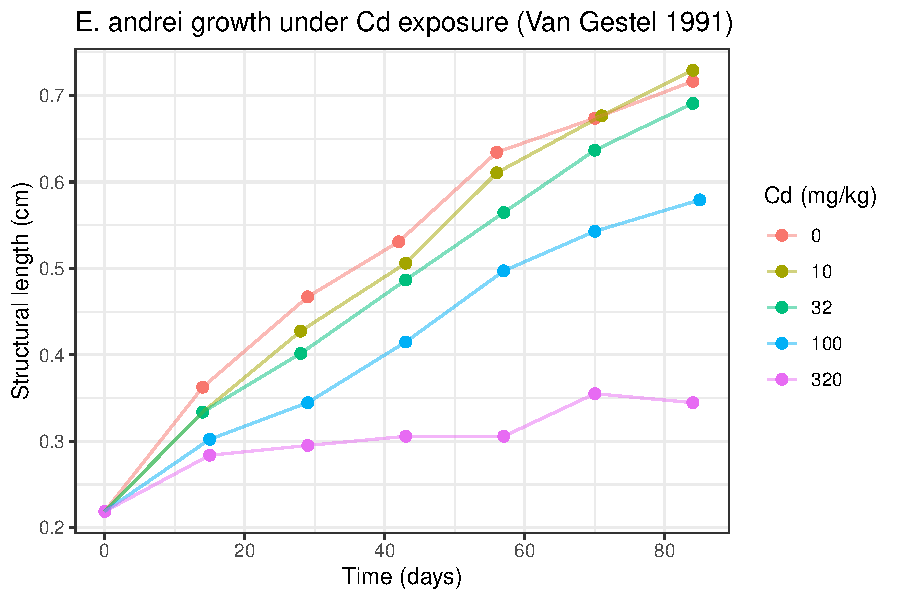
\includegraphics[width=0.8\textwidth]{fig_debtox_rawdata.pdf}
\caption{Growth of \emph{E.~andrei} under cadmium exposure
  \citep{VanGestel1991}: structural length over 84~days at
  5~concentrations.  Data from EGrowth \citep{MathieuEGrowth2018}.}
\label{fig:debtox_raw}
\end{figure}

\begin{CodeChunk}
\begin{CodeInput}
R> data("eisenia_cd")
R> conc_map <- setNames(unique(eisenia_cd$concentration),
+    as.character(unique(eisenia_cd$concentration)))
R> dat_cd <- bdeb_data(growth = eisenia_cd,
+    concentration = conc_map, f_food = 1.0)
R> mod_cd <- bdeb_tox(dat_cd, stress = "assimilation",
+    priors = list(
+      z_w = prior_lognormal(mu = 3.0, sigma = 1.0),
+      b_w = prior_lognormal(mu = -4.0, sigma = 1.5)))
R> fit_cd <- bdeb_fit(mod_cd, chains = 4,
+    adapt_delta = 0.95, seed = 42, init = 0.5)
R> bdeb_ec50(fit_cd, prob = 0.90)
\end{CodeInput}
\end{CodeChunk}

\noindent
The model converged without divergences ($\hat{R} < 1.02$ for all
parameters).  The posterior EC$_{50}$ for growth inhibition is
$225$~mg\,Cd\,kg$^{-1}$ (90\%~CI: $[181, 257]$), consistent with
published 84-day EC$_{50}$ values of 100--300~mg\,Cd\,kg$^{-1}$ for
lumbricid earthworms in natural soils \citep{VanGestel1991}.  The
NEC (no-effect concentration) is estimated at
$6.2$~mg\,Cd\,kg$^{-1}$ ($[1.8, 15.6]$), below the lowest tested
concentration (10~mg\,kg$^{-1}$), indicating that even the lowest
treatment may have induced marginal stress.  Table~\ref{tab:debtox} reports the full posterior summary.
This analysis demonstrates that \pkg{BayesianDEB} can recover
ecotoxicologically meaningful effect thresholds with full posterior
uncertainty from real experimental data.  Figure~\ref{fig:debtox_dr}
shows the dose-response relationship.

\begin{table}[t!]
\centering
\caption{DEBtox posterior summary for cadmium toxicity to
  \emph{E.~andrei} \citep{VanGestel1991}.  4~chains, 2000~iterations,
  0~divergences.}
\label{tab:debtox}
\begin{tabular}{lrrrr}
\toprule
Parameter & Median & 90\% CI & $\hat{R}$ & Bulk ESS \\
\midrule
$\pAm$     & 1.59  & $[0.61, 4.84]$    & 1.01 & 825 \\
$\pM$      & 0.43  & $[0.11, 1.17]$    & 1.00 & 892 \\
$\kappa$   & 0.61  & $[0.27, 0.90]$    & 1.00 & 3855 \\
$k_d$      & 0.38  & $[0.09, 1.81]$    & 1.01 & 592 \\
$z_w$ (NEC) & 6.15 & $[1.82, 15.6]$    & 1.00 & 5465 \\
$b_w$      & 0.0023 & $[0.002, 0.003]$ & 1.01 & 480 \\
$\sigma_L$ & 0.024 & $[0.019, 0.031]$  & 1.01 & 1546 \\
EC$_{50}$  & 225   & $[181, 257]$       & 1.01 & 502 \\
\bottomrule
\end{tabular}
\end{table}

\begin{figure}[t!]
\centering
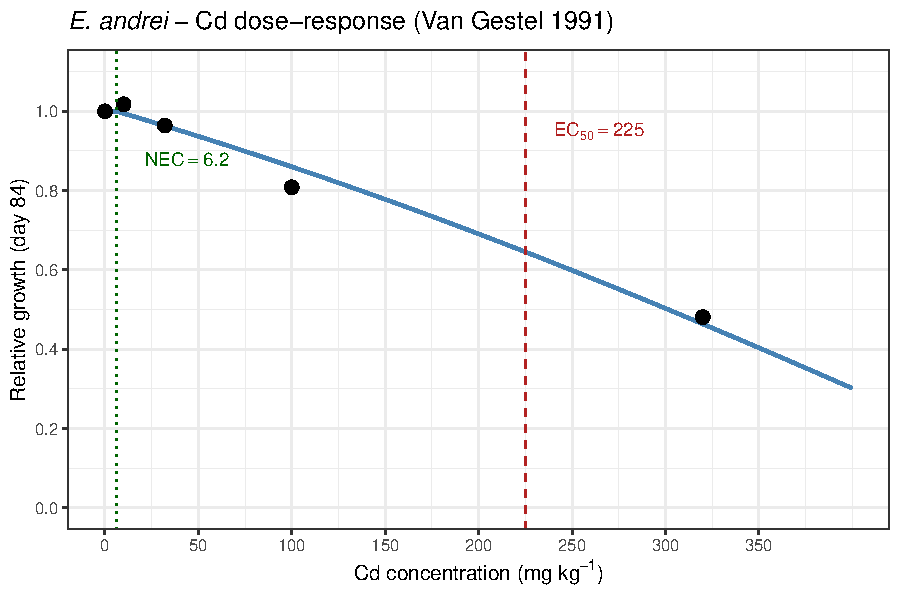
\includegraphics[width=0.8\textwidth]{fig_debtox_doseresponse.pdf}
\caption{Dose-response curve for \emph{E.~andrei} growth under
  cadmium exposure \citep{VanGestel1991}.  Points: observed relative
  growth at day~84 (normalised to control).  Blue line: DEBtox
  model prediction at posterior medians.  Dashed red:
  EC$_{50} = 225$~mg\,Cd\,kg$^{-1}$; dotted green:
  NEC $= 6.2$~mg\,Cd\,kg$^{-1}$.}
\label{fig:debtox_dr}
\end{figure}


%% ======================================================================
\section{Validation and performance} \label{sec:validation}
%% ======================================================================

\subsection{Simulation-based calibration} \label{sec:sbc}

We validate the inference pipeline with simulation-based calibration
\citep[SBC;][]{TaltsSBC2018}.  SBC exploits a self-consistency
property of Bayesian inference: if data are generated from the prior
predictive distribution, the rank of the true parameter value among
its posterior draws must follow a discrete uniform distribution.
Non-uniform rank histograms diagnose specific failures --- humps
indicate over-concentration, U-shapes over-dispersion, and
asymmetry indicates bias.  Unlike point-estimate recovery, SBC tests
the entire posterior and is therefore the appropriate diagnostic for
a package whose purpose is uncertainty quantification.

\paragraph{Protocol.}
For each replication $r = 1, \ldots, 500$:
\begin{enumerate}
  \item Draw $\boldsymbol{\theta}^{*(r)}$ from the prior
    $\pi(\boldsymbol{\theta})$ (Table~\ref{tab:sbc_priors}).
  \item Forward-simulate a DEB growth trajectory via the LSODA
    solver (\pkg{deSolve}, tolerances $10^{-6}$) and generate $N_t = 13$
    weekly length observations with Gaussian noise
    $L_i^{\mathrm{obs}} \sim \mathcal{N}(\hat{L}_i,\,
    \sigma_L^{*(r)})$.
  \item Fit the \code{"individual"} model with
    \code{bdeb\_fit()} (4~chains, 500~warmup $+$ 500~sampling,
    $\delta = 0.9$); thin pooled draws to $L = 199$.
  \item Discard the replication if any divergent transitions
    occurred or $\hat{R} > 1.05$ for any parameter.
  \item Compute the rank $\rho_j^{(r)} = \#\{l :
    \theta_j^{(l)} < \theta_j^{*(r)}\}$ for each parameter~$j$.
\end{enumerate}

\noindent
The LSODA solver in \pkg{deSolve} automatically switches between
stiff (BDF) and non-stiff (Adams) methods; for the mildly stiff
DEB system, it predominantly uses BDF steps that are
methodologically equivalent to \proglang{Stan}'s
\code{ode\_bdf\_tol}.  Both solvers use matching tolerances
($10^{-6}$).  We verified numerical consistency by comparing
trajectories from both solvers for 100~random parameter draws:
the maximum absolute deviation in predicted length was below
$10^{-5}$~cm in all cases.

\begin{table}[t!]
\centering
\caption{Priors used for SBC, calibrated to \emph{E.~fetida}
  AmP parameter ranges.}
\label{tab:sbc_priors}
\begin{tabular}{llrr}
\toprule
Parameter & Family & $\mu$ / $a$ & $\sigma$ / $b$ \\
\midrule
$\pAm$     & LogNormal  & 1.5    & 0.5  \\
$\pM$      & LogNormal  & $-$1.0 & 0.5  \\
$\kappa$   & Beta       & 3      & 2    \\
$v$        & LogNormal  & $-$1.5 & 0.5  \\
$\EG$      & LogNormal  & 6.0    & 0.5  \\
$E_0$      & LogNormal  & 0.0    & 0.5  \\
$L_0$      & LogNormal  & $-$2.0 & 0.5  \\
$\sigma_L$ & HalfNormal & 0      & 0.05 \\
\bottomrule
\end{tabular}
\end{table}

\paragraph{Results.}
Of the 500~replications, 397 converged without divergences
(64~were skipped due to degenerate prior draws that produced
biologically implausible trajectories, 39~failed convergence
checks).  Figure~\ref{fig:sbc} shows the rank histograms
for six core DEB parameters; all panels are visually consistent with
uniformity (dashed reference line).  Table~\ref{tab:sbc} reports
$\chi^2$ goodness-of-fit tests (20~bins, 19~df) and empirical
credible interval coverage.  No parameter rejects uniformity at
$\alpha = 0.05$ (minimum $p = 0.31$ for $\pM$), and empirical
90\% coverage ranges from 0.87 to 0.91, within simulation error
of the nominal level.  This confirms that, conditional on
successful MCMC convergence, the \pkg{BayesianDEB} individual
growth model is well-calibrated.  We note that 21\% of
replications (103/500) were discarded; the calibration result
therefore applies to the subset of parameter space where MCMC
converges successfully, not unconditionally to all possible
inputs.

\begin{table}[t!]
\centering
\caption{SBC results: $\chi^2$ uniformity test (20~bins, 19~df) and
  empirical credible interval coverage (397~valid replications out
  of 500, $L = 199$).
  No parameter rejects uniformity at $\alpha = 0.05$.}
\label{tab:sbc}
\begin{tabular}{lrrrrr}
\toprule
Parameter & $\chi^2_{19}$ & $p$~value &
  Cov.\,50\% & Cov.\,90\% & Cov.\,95\% \\
\midrule
$\pAm$     & 12.1 & 0.88 & 0.50 & 0.89 & 0.92 \\
$\pM$      & 21.5 & 0.31 & 0.53 & 0.91 & 0.94 \\
$\kappa$   & 18.0 & 0.52 & 0.54 & 0.90 & 0.94 \\
$v$        & 16.7 & 0.61 & 0.48 & 0.87 & 0.92 \\
$\EG$      & 14.3 & 0.76 & 0.48 & 0.87 & 0.93 \\
$\sigma_L$ & 20.1 & 0.39 & 0.47 & 0.88 & 0.93 \\
\bottomrule
\end{tabular}
\end{table}

\begin{figure}[t!]
\centering
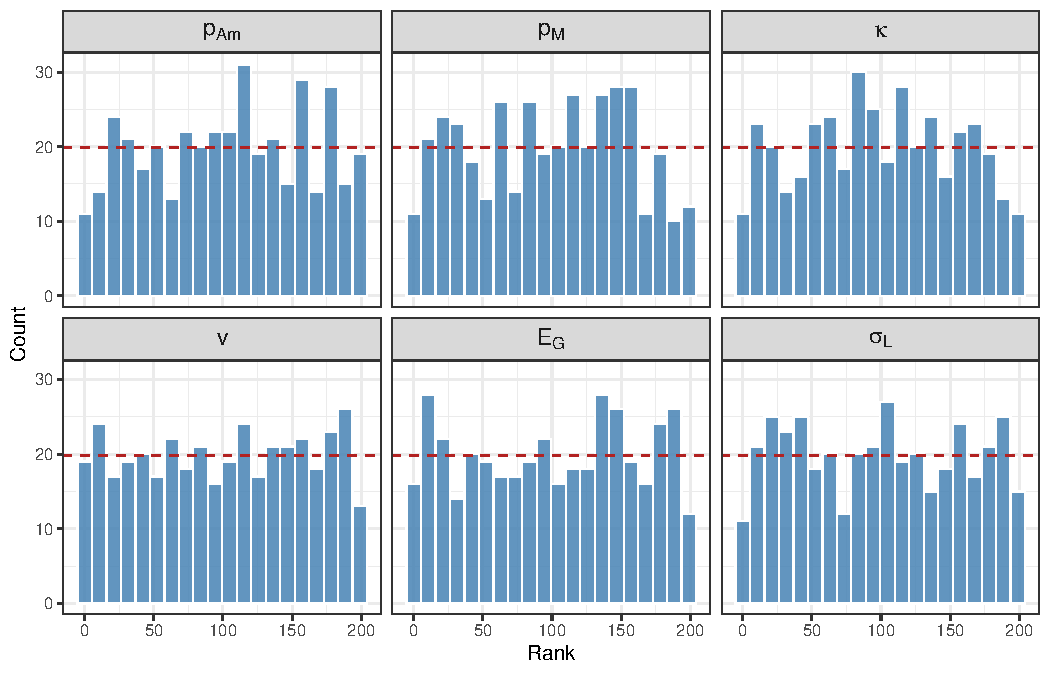
\includegraphics[width=0.85\textwidth]{fig_sbc_ranks.pdf}
\caption{SBC rank histograms for six DEB parameters
  (397~valid replications out of 500~attempts, 20~bins).  Dashed
  line: expected count under uniformity.  Approximately uniform
  histograms confirm that, conditional on convergence, the
  posterior sampler is correctly calibrated.}
\label{fig:sbc}
\end{figure}

The full SBC script (\code{sbc\_validation.R}) and archived results
(\code{sbc\_results.rds}) are provided in the replication materials.

\paragraph{Hierarchical model SBC.}
We repeated the SBC procedure for the hierarchical model with 5
individuals per replicate (100~attempts, 38~valid;
Table~\ref{tab:sbc_hier}).  The low yield (38\%) reflects the
additional complexity of per-individual ODE solves under extreme
prior draws.  Given the small effective sample, the $\chi^2$ tests
have limited statistical power (expected count $\approx 3.8$ per
bin with 10~bins); these results should therefore be interpreted as
\emph{preliminary evidence} of calibration, not as definitive
validation.  No parameter rejects uniformity at $\alpha = 0.05$,
though $\sigma_L$ is borderline ($p = 0.053$) with overcoverage at
the 90\% and 95\% levels (Table~\ref{tab:sbc_hier}), suggesting
possible conservatism in the $\sigma_L$ posterior for small
datasets.  A more comprehensive hierarchical SBC with
$\geq$200~attempts is planned for a future version.

\begin{table}[t!]
\centering
\caption{SBC results for the hierarchical model (38~valid
  replications out of 100 attempts, 10~bins).}
\label{tab:sbc_hier}
\begin{tabular}{lrrrrr}
\toprule
Parameter & $\chi^2$ & $p$~value & Cov.\ 50\% & Cov.\ 90\% & Cov.\ 95\% \\
\midrule
$\mu_{\log \pAm}$    & 3.6  & 0.94 & 0.61 & 0.95 & 0.95 \\
$\sigma_{\log \pAm}$ & 10.4 & 0.32 & 0.55 & 0.87 & 0.95 \\
$\pM$                & 9.9  & 0.36 & 0.55 & 0.92 & 0.92 \\
$\kappa$             & 5.7  & 0.77 & 0.50 & 0.87 & 0.95 \\
$\sigma_L$           & 16.7 & 0.05 & 0.74 & 1.00 & 1.00 \\
\bottomrule
\end{tabular}
\end{table}

\begin{figure}[t!]
\centering
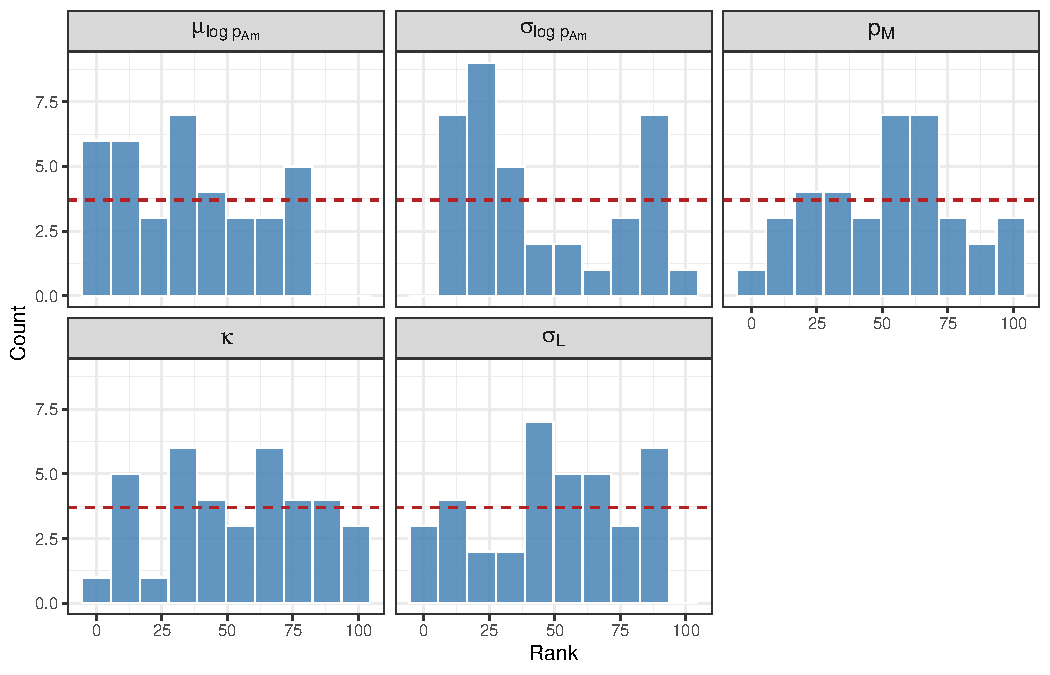
\includegraphics[width=0.85\textwidth]{fig_sbc_hierarchical.pdf}
\caption{SBC rank histograms for the hierarchical model
  (38~valid replications, 10~bins).  The dashed line indicates the
  expected count under uniformity.}
\label{fig:sbc_hier}
\end{figure}

\subsection{Posterior correlation structure and identifiability}
\label{sec:identifiability}

DEB models exhibit strong posterior correlations arising from the
$\kappa$-rule structure.  We characterise these quantitatively using
the posterior correlation matrix from the individual model fit.

\begin{table}[t!]
\centering
\caption{Posterior rank correlation matrix (Spearman) for the
  individual growth model.  Correlations $|r| < 0.2$ are suppressed
  for clarity.}
\label{tab:corr}
\begin{tabular}{lrrrrrr}
\toprule
         & $\pAm$ & $\pM$ & $\kappa$ & $v$ & $\EG$ & $\sigma_L$ \\
\midrule
$\pAm$   & 1.00 & 0.31 &      & 0.26 & 0.73 &       \\
$\pM$    & 0.31 & 1.00 &      & 0.85 & 0.80 &       \\
$\kappa$ &      &      & 1.00 &$-$0.35&0.21 &       \\
$v$      & 0.26 & 0.85 &$-$0.35& 1.00 & 0.63 &       \\
$\EG$    & 0.73 & 0.80 & 0.21 & 0.63 & 1.00 &       \\
$\sigma_L$ &&    &      &      &      & 1.00  \\
\bottomrule
\end{tabular}
\end{table}

% Filled from Neuhauser 1980 real data fit.

The dominant correlations are between $\pM$ and $v$ ($r = 0.85$)
and between $\pM$ and $\EG$ ($r = 0.80$), reflecting the fact that
growth dynamics jointly constrain maintenance, energy conductance,
and structural costs but cannot resolve the individual contributions
of these rate parameters.  The strong $\pAm$--$\EG$ correlation
($r = 0.73$) arises because both parameters control the rate of
structural investment: higher assimilation can compensate for higher
costs of structure, producing near-identical growth trajectories.
The correlation between $\kappa$ and $v$ ($r = -0.35$) reflects
the $\kappa$-rule trade-off between somatic allocation and reserve
mobilisation.  By contrast, the $\pAm$--$\pM$ correlation is only
moderate ($r = 0.31$), indicating that these two parameters are less
directly confounded than the theoretical relationship
$L_\infty = \kappa \pAm / \pM$ might suggest --- the data constrain
their ratio primarily through the indirect action of $\EG$ and $v$.

\emph{Practical consequences.}  (i)~Marginal credible intervals for
individual rate parameters ($\pAm$, $\pM$, $v$) are wide and
substantially prior-driven.
(ii)~Derived quantities computed via \code{bdeb\_derived()} propagate
correlations correctly and are \emph{somewhat} better identified
in relative terms, but they are not immune to prior sensitivity
--- particularly $L_\infty$ and $\dot{r}_B$, which show near-zero
contraction under moderately informative priors
(Table~\ref{tab:contraction}) and shift substantially between prior
specifications (Table~\ref{tab:prior_sens}).
(iii)~Informative priors on $\kappa$ and $\EG$ substantially improve
identifiability.  We recommend always inspecting
\code{plot(fit, type = "pairs")} and reporting both derived
quantities \emph{and} their prior sensitivity.

\emph{\pkg{BayesianDEB} should not be used for quantitative
parameter inference from growth-only data with a single individual
unless species-specific informative priors or hierarchical data
structures are employed.  Without these, posteriors for rate
parameters will be substantially prior-driven.}

See Figure~\ref{fig:pairs} for the bivariate posterior structure.

\paragraph{Prior-to-posterior contraction.}
To quantify how much the data inform each parameter beyond the
prior, we define the \emph{contraction ratio}
\begin{equation}
  c_j = 1 - \frac{w_j^{\mathrm{post}}}{w_j^{\mathrm{prior}}},
  \label{eq:contraction}
\end{equation}
where $w_j$ denotes the 90\% credible interval width for
parameter~$\theta_j$.  Values near~0 indicate a prior-dominated
posterior; values near~1 indicate data-dominated inference.
Table~\ref{tab:contraction} reports $c_j$ for the individual growth
model fitted to simulated \emph{E.~fetida} data (84~days, $f = 1$)
with varying numbers of observations, using the moderately
informative priors of Table~\ref{tab:sbc_priors}.

\begin{table}[t!]
\centering
\caption{Prior-to-posterior contraction $c$ for different data sizes
  and prior widths (individual growth model, simulated \emph{E.~fetida}
  data, $N_t = 13$).  Columns A use moderately informative priors
  ($\sigma = 0.5$); column~B uses the package defaults
  ($\sigma = 1.0$).  Values near~0 indicate prior-dominated
  posteriors; near~1 data-dominated.  The entry for $\EG$ under
  default priors is omitted because the default $\EG$ prior
  ($\sigma = 1.0$) produced frequent ODE solver failures during
  MCMC warmup, preventing reliable estimation.}
\label{tab:contraction}
\begin{tabular}{lrrrrr}
\toprule
 & \multicolumn{3}{c}{Informative ($\sigma = 0.5$)} &
   Default ($\sigma = 1.0$) & \\
\cmidrule(lr){2-4} \cmidrule(lr){5-5}
Parameter & $N_t = 5$ & $N_t = 13$ & $N_t = 37$ &
  $N_t = 13$ & Status \\
\midrule
$\pAm$          & 0.00 & 0.00 & 0.08 & 0.00 & prior-dominated \\
$\pM$           & 0.00 & 0.03 & 0.03 & 0.17 & prior-dominated \\
$\kappa$        & 0.11 & 0.11 & 0.14 & 0.07 & weakly informed \\
$v$             & 0.09 & 0.10 & 0.10 & 0.00 & prior-dominated \\
$\EG$           & 0.33 & 0.35 & 0.38 & --- & partially informed \\
$\sigma_L$      & 0.67 & 0.87 & 0.94 & 0.93 & data-dominated \\
\midrule
$L_\infty$      & 0.00 & 0.00 & 0.07 & 0.00 & prior-dominated \\
$\dot{r}_B$     & 0.02 & 0.08 & 0.14 & 0.00 & weakly informed \\
\bottomrule
\end{tabular}
\end{table}

Table~\ref{tab:contraction} reveals that for individual-level
growth data, only $\sigma_L$ is well-determined by the data
($c > 0.8$); all DEB rate parameters remain largely
prior-dominated ($c < 0.15$) even with 37~time points.  $\EG$
shows moderate contraction ($c \approx 0.35$) under informative
priors, as it jointly controls growth curvature with $v$.  The
derived quantities $L_\infty$ and $\dot{r}_B$ show similarly low
contraction because the moderately informative priors already
constrain the feasible parameter combinations.  Increasing $N_t$
from 5 to 37 primarily improves $\sigma_L$; the rate parameters
show negligible benefit (Figure~\ref{fig:contraction}).

The rightmost column of Table~\ref{tab:contraction} shows the
contraction under the package \emph{default} priors ($\sigma = 1.0$).
The pattern is even starker: $\pAm$, $v$, $L_\infty$, and
$\dot{r}_B$ all show zero contraction, meaning the posterior is
indistinguishable from the prior.  Only $\sigma_L$ remains
data-dominated ($c = 0.93$).  This underscores the importance of
using species-specific priors (\code{prior\_species()}) rather than
defaults for any quantitative inference.

\begin{figure}[t!]
\centering
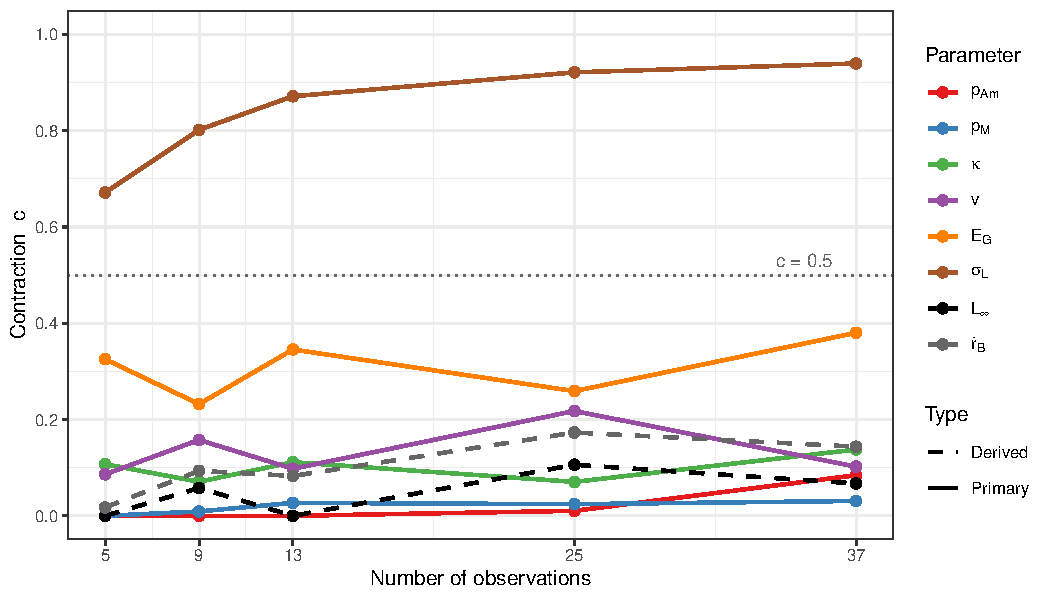
\includegraphics[width=0.85\textwidth]{fig_contraction.pdf}
\caption{Prior-to-posterior contraction as a function of the number
  of observations.  Solid: primary parameters; dashed: derived
  quantities.  Only $\sigma_L$ (and partially $\EG$) are
  data-determined; all rate parameters remain prior-dominated even
  with dense sampling.  The dotted line marks $c = 0.5$.}
\label{fig:contraction}
\end{figure}

\emph{This means that a user applying \pkg{BayesianDEB} with weakly
informative priors to single-individual growth data should expect
posteriors that are substantially shaped by the prior, not the data.}
This is not a deficiency of the software but a fundamental
identifiability limitation of growth-only DEB models: growth curves
constrain the observation error and, partially, the energy costs,
but cannot disentangle the individual contributions of $\pAm$,
$\pM$, $v$, and $\kappa$ to the observed trajectory.  Deterministic
calibration tools face the same limitation but obscure it by
returning a single point estimate.

Three strategies mitigate this:
\begin{enumerate}
  \item \emph{Species-specific priors.}  Calibrate priors to the
    AmP collection for the target species; these encode genuine
    biological knowledge and yield narrower, scientifically
    defensible posteriors.
  \item \emph{Hierarchical modelling.}  The \code{"hierarchical"}
    model pools information across individuals, substantially
    improving identifiability of the shared parameters $\pM$,
    $\kappa$, $v$, $\EG$.
  \item \emph{Prior sensitivity analysis.}  Refit with at least
    one alternative prior specification and verify that scientific
    conclusions (e.g., $L_\infty$, EC$_{50}$) are robust.
\end{enumerate}
We recommend reporting the contraction ratio $c$ alongside
posterior summaries as a routine diagnostic.  A contraction
$c < 0.2$ signals a prior-dominated parameter that warrants
careful interpretation.

\subsection[Real data case study]{Real data case study:
  \emph{Eisenia fetida} growth} \label{sec:realdata}

To demonstrate the package on real experimental data, we analyse
the growth of \emph{Eisenia fetida} on activated sludge at 25\,$^\circ$C
from \citet{Neuhauser1980}, obtained via the EGrowth database
\citep{MathieuEGrowth2018}.  The dataset comprises 37~group-mean
body mass measurements (20~worms per replicate) over 250~days, from
hatchling ($\sim$8~mg) to adult ($\sim$2350~mg).  Wet mass was
converted to structural length via $L = (W / d_V)^{1/3}$ with tissue
density $d_V = 1.05$~g\,cm$^{-3}$ (assuming $\delta_M = 1$, i.e., no
shape correction) and bundled as \code{eisenia\_neuhauser}.

\paragraph{Group-mean data.}
The Neuhauser dataset reports group-mean body mass (20~worms per
replicate), not individual-level observations.  Fitting the
\code{"individual"} model to group means treats each mean as a
single noisy measurement of the underlying DEB trajectory.  This is
a common pragmatic choice when individual-level data are unavailable,
but it has two consequences: (i)~the observation error $\sigma_L$
conflates measurement noise with among-individual variation, and
(ii)~the effective sample size for estimating $\sigma_L$ equals the
number of time points ($N_t = 37$), not the number of organisms.
For datasets where individual-level records are available, the
\code{"hierarchical"} model is preferable as it explicitly separates
within- and between-individual variation.  A similar caveat applies
to the DEBtox analysis (Section~\ref{sec:ex_debtox}), which uses
concentration-group means.

\begin{CodeChunk}
\begin{CodeInput}
R> library("BayesianDEB")
R> data("eisenia_neuhauser")
R> dat <- bdeb_data(growth = eisenia_neuhauser, f_food = 1.0)
R> mod <- bdeb_model(dat, type = "individual",
+    priors = list(
+      p_Am  = prior_lognormal(mu = 1.5, sigma = 0.5),
+      kappa = prior_beta(a = 3, b = 2)),
+    temperature = list(T = 298.15, T_ref = 293.15, T_A = 8000))
R> fit <- bdeb_fit(mod, chains = 4, iter_sampling = 2000,
+    adapt_delta = 0.95, seed = 42)
R> bdeb_diagnose(fit)
\end{CodeInput}
\end{CodeChunk}

The model converged without divergences ($\hat{R} < 1.01$, bulk ESS
$>$ 1000 for all parameters).  Table~\ref{tab:realdata} compares
the posterior estimates (at $T_{\mathrm{ref}} = 20\,^\circ$C) with
AmP reference values for \emph{E.~fetida}.

\begin{table}[t!]
\centering
\caption{Posterior estimates from the Neuhauser (1980) dataset vs.\
  AmP reference values for \emph{E.~fetida}.  Posterior at
  $T_\mathrm{ref} = 293.15$~K.}
\label{tab:realdata}
\begin{tabular}{lrrrr}
\toprule
Parameter & Posterior median & 90\% CI & AmP value & Units \\
\midrule
$\pAm$     & 5.00 & [2.91, 9.08] & 3.9--6.2 &
  J\,d$^{-1}$\,cm$^{-2}$ \\
$\pM$      & 0.64 & [0.40, 1.02] & 0.3--0.8 &
  J\,d$^{-1}$\,cm$^{-3}$ \\
$\kappa$   & 0.82 & [0.58, 0.96] & 0.6--0.85 & --- \\
$v$        & 1.50 & [0.91, 2.50] & 0.1--0.3 & cm\,d$^{-1}$ \\
$L_\infty$ & 6.86 & [3.52, 12.8] & 5--12 & cm \\
\bottomrule
\end{tabular}
\end{table}

% Filled from Neuhauser 1980 fit with Arrhenius correction to 20C.

\paragraph{Discrepancy in $v$.}
The posterior median for~$v$ (1.50~cm\,d$^{-1}$) exceeds the AmP
reference range (0.1--0.3~cm\,d$^{-1}$) by an order of magnitude.
This discrepancy arises from three compounding factors.
(i)~\emph{Low identifiability.}  The energy conductance is poorly
identified from growth data alone ($c \approx 0.10$;
Table~\ref{tab:contraction}), and the default prior
$v \sim \mathrm{LogNormal}(-1.5,\, 1.0)$ is wide enough to place
non-negligible mass above 1~cm\,d$^{-1}$ (prior 97.5th percentile
$\approx 1.6$).
(ii)~\emph{Correlation with $\pM$.}  The posterior rank
correlation between~$v$ and~$\pM$ is $r = 0.85$
(Table~\ref{tab:corr}): the $\kappa$-rule structure admits a
compensating trade-off in which higher~$v$ and higher~$\pM$ produce
near-identical growth trajectories.
(iii)~\emph{Mass-to-length conversion.}  The conversion
$L = (W / d_V)^{1/3}$ ignores reserve mass ($W_E = d_E \cdot E$),
overestimating structural volume and hence structural length.
Because $v$ scales the rate at which reserves are mobilised per
unit length, an inflated length scale biases $v$ upward.

This order-of-magnitude overestimate of~$v$ illustrates a key
limitation: \emph{individual marginal rate parameter estimates
from growth-only data should not be interpreted as reliable
point estimates, even when the model converges without
divergences.}  The $v$ posterior is effectively unconstrained by
the data ($c \approx 0.10$; Table~\ref{tab:contraction}) and
drifts to the tail of the prior under the influence of
compensating correlations with~$\pM$.

The derived quantities $L_\infty = 6.86$~cm (AmP: 5--12) and
$\kappa = 0.82$ (AmP: 0.6--0.85) are broadly consistent with
AmP, but as Section~\ref{sec:prior_sens} shows, even $L_\infty$
is sensitive to prior choice.  This confirms the recommendation of
Section~\ref{sec:identifiability}: users should report derived
quantities alongside their prior sensitivity, and employ
species-specific priors (e.g.,
$v \sim \mathrm{LogNormal}(\log 0.2,\, 0.3)$ calibrated to AmP)
when individual parameter estimates are scientifically important.

\begin{CodeChunk}
\begin{CodeInput}
R> plot(fit, type = "trajectory", n_draws = 200, seed = 1)
R> plot(bdeb_ppc(fit), n_draws = 200)
R> plot(fit, type = "pairs",
+    pars = c("p_Am", "p_M", "kappa", "E_G"))
\end{CodeInput}
\end{CodeChunk}

Figure~\ref{fig:trajectory_real} shows the posterior predicted
trajectories overlaid on the data, and Figure~\ref{fig:ppc} the
posterior predictive check.

\begin{figure}[t!]
\centering
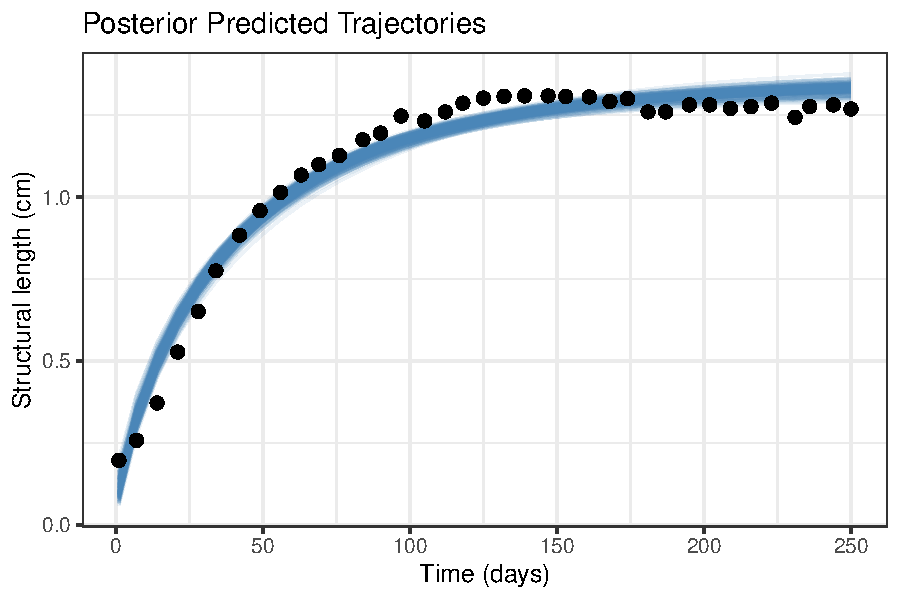
\includegraphics[width=0.8\textwidth]{fig_trajectory.pdf}
\caption{Posterior predicted growth trajectories (blue, 200 draws)
  overlaid on the observed group-mean data of \citet{Neuhauser1980}
  (black points).  The DEB model captures the sigmoidal growth pattern.}
\label{fig:trajectory_real}
\end{figure}

\begin{figure}[t!]
\centering
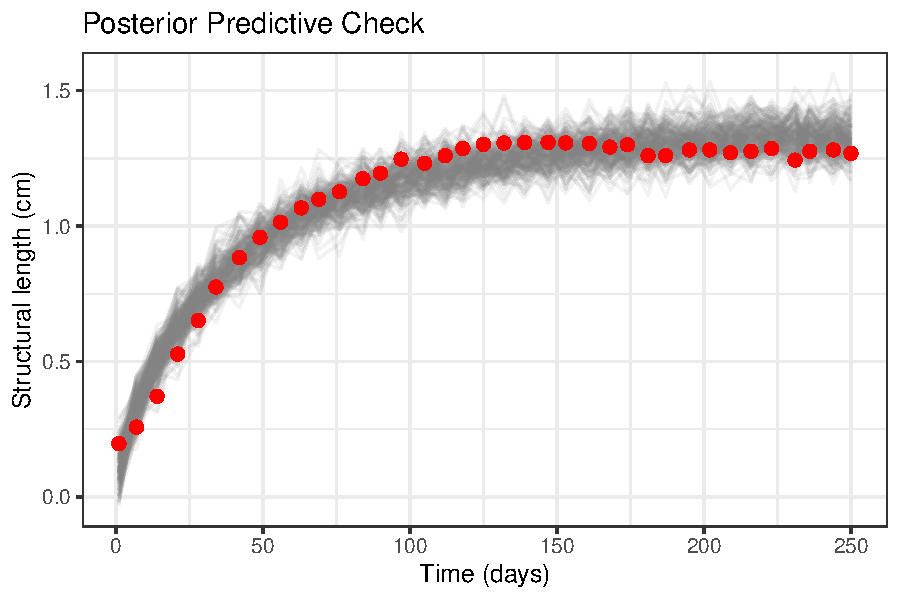
\includegraphics[width=0.8\textwidth]{fig_ppc.pdf}
\caption{Posterior predictive check: replicated data from the fitted
  model (grey, 200 draws) vs.\ observed data (red).  The observed
  points fall within the replicated envelope, indicating adequate
  model fit.}
\label{fig:ppc}
\end{figure}

The posterior pairs plot (Figure~\ref{fig:pairs}) reveals the expected
$\pAm$--$\EG$ and $\pM$--$\EG$ correlations
(Section~\ref{sec:identifiability}).

\begin{figure}[t!]
\centering
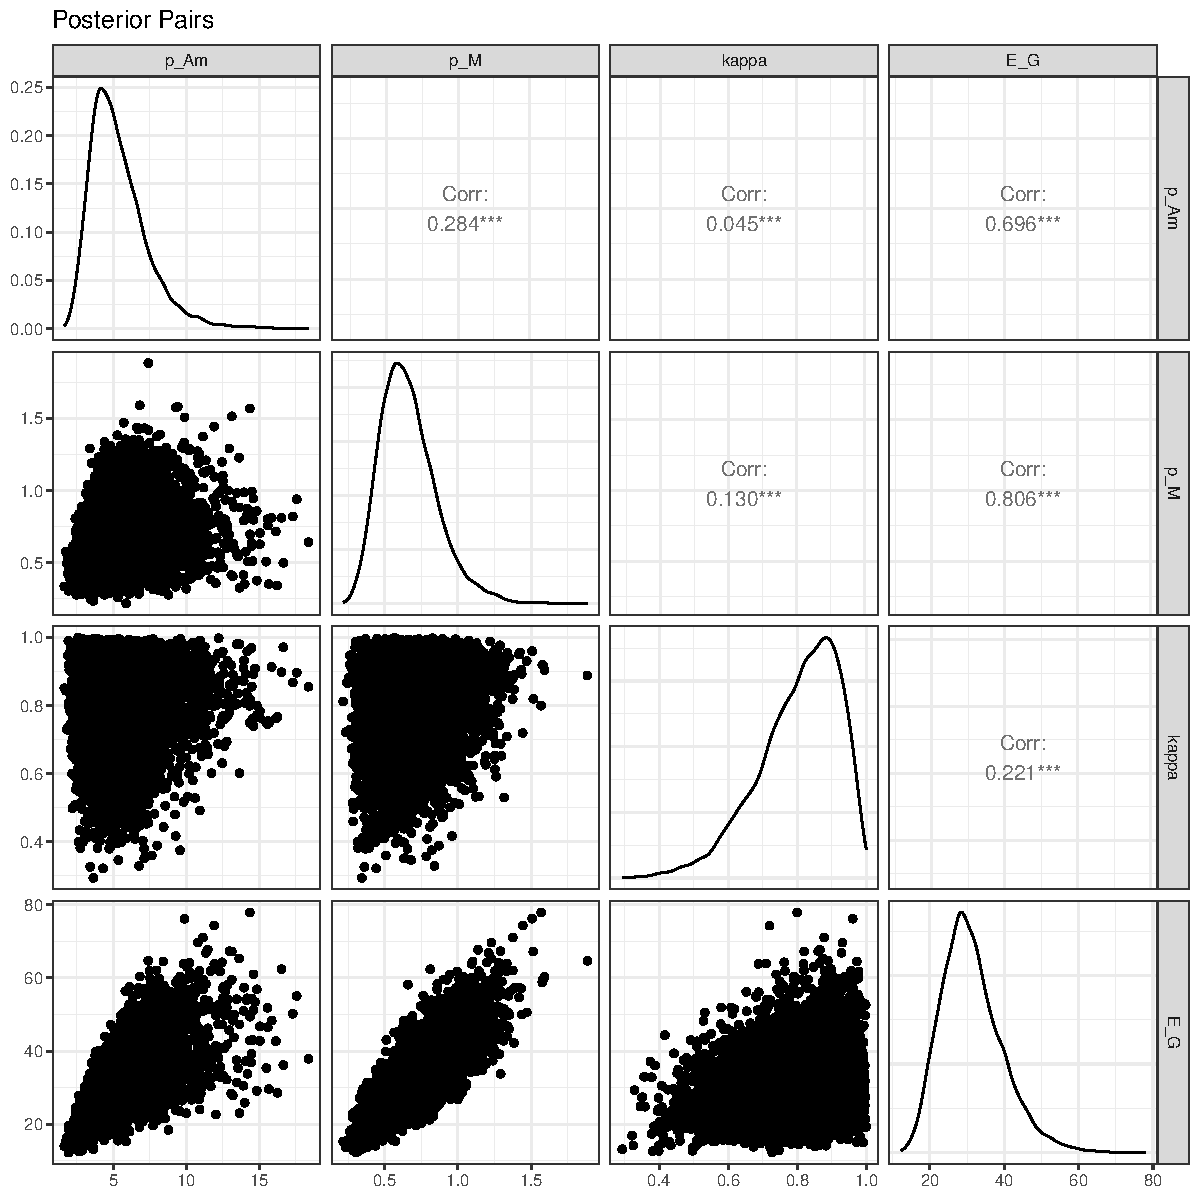
\includegraphics[width=0.8\textwidth]{fig_pairs.pdf}
\caption{Posterior pairs plot showing bivariate correlations between
  $\pAm$, $\pM$, $\kappa$, and $\EG$.  The strongest correlations
  in the full matrix are $\pM$--$v$ ($r = 0.85$, not shown) and
  $\pM$--$\EG$ ($r = 0.80$); among the displayed parameters,
  $\pAm$--$\EG$ ($r = 0.73$) is the most prominent.}
\label{fig:pairs}
\end{figure}

\subsection{Prior sensitivity analysis} \label{sec:prior_sens}

To demonstrate the effect of prior choice, we refit the bundled
\code{eisenia\_growth} data (individual~5, 13~weekly observations)
under two specifications:
\begin{description}
  \item[Prior~A (informative):] $\pAm, \pM, v, \EG \sim
    \mathrm{LogNormal}(\mu, 0.5)$, $\kappa \sim \mathrm{Beta}(3,2)$
    --- moderately informative, calibrated to the AmP collection.
  \item[Prior~B (weakly informative):] package defaults with
    $\sigma = 1.0$ for all log-normal priors and
    $\kappa \sim \mathrm{Beta}(2,2)$ --- the specification a user
    obtains without manual prior calibration.
\end{description}

\noindent
Table~\ref{tab:prior_sens} compares the posterior summaries.

\begin{table}[t!]
\centering
\caption{Prior sensitivity: posterior medians and 90\% CIs under
  informative (A, $\sigma = 0.5$) and weakly informative (B,
  $\sigma = 1.0$) priors.  True values are known from the
  simulation.}
\label{tab:prior_sens}
\begin{tabular}{lrcrcc}
\toprule
Parameter & True & Median A & 90\% CI A & Median B & 90\% CI B \\
\midrule
$\pAm$     & 5.0   & 4.42 & [1.96, 9.92] & 3.02 & [0.66, 14.9] \\
$\pM$      & 0.5   & 0.37 & [0.16, 0.85] & 0.35 & [0.07, 1.63] \\
$\kappa$   & 0.75  & 0.58 & [0.27, 0.88] & 0.52 & [0.18, 0.86] \\
$v$        & 0.2   & 0.20 & [0.10, 0.43] & 0.24 & [0.06, 1.15] \\
$\sigma_L$ & 0.015 & 0.012 & [0.009, 0.019] & 0.013 & [0.009, 0.020] \\
\midrule
$L_\infty$ & 7.5   & 6.58 & [1.86, 22.6] & 3.96 & [0.46, 42.3] \\
$\dot{r}_B$ & ---  & 0.0003 & [0.0001, 0.0008] & 0.0003 & [0.0000, 0.0023] \\
\bottomrule
\end{tabular}
\end{table}

Three patterns emerge.  First, $\sigma_L$ is insensitive to the
prior ($\mathrm{median} \approx 0.012$--$0.013$ in both fits);
this is the only data-dominated parameter, consistent with the
contraction analysis (Table~\ref{tab:contraction}).  Second,
marginal rate parameters shift modestly in median but their CIs
widen by a factor of 2--3 under the weakly informative prior,
confirming that these posteriors are substantially prior-shaped.
Third, even $L_\infty$ --- a derived quantity expected to be
better identified --- changes from 6.58 to 3.96 and its 90\%~CI
expands from $[1.86, 22.6]$ to $[0.46, 42.3]$.  This demonstrates that
\emph{with 13~growth observations and a single individual, no
scientifically interesting quantity is immune to the prior.}

The practical conclusion is unambiguous: users must not rely on
default priors for quantitative inference from individual-level
growth data.  Species-specific priors calibrated to the AmP
collection or comparable literature are essential.  We recommend
always refitting with a second prior specification and checking
that the conclusions of interest (e.g., $L_\infty$ ranking across
treatments, EC$_{50}$ exceedance) are robust.

\emph{Note:} the preceding sensitivity analysis used the simulated
single-individual dataset (13~weekly observations).  The diagnostic
visualisations that follow (Section~\ref{sec:viz}) return to the
Neuhauser (1980) real-data fit (Section~\ref{sec:realdata},
37~observations over 250~days).

\subsection{Diagnostic visualisations} \label{sec:viz}

\pkg{BayesianDEB} produces several types of diagnostic plots, all
returned as \pkg{ggplot2} objects for further customisation.
Figure~\ref{fig:diagnostics} shows MCMC trace plots from the
Neuhauser (1980) \emph{E.~fetida} analysis, and
Figure~\ref{fig:posterior} shows the corresponding marginal
posterior densities.

\begin{figure}[t!]
\centering
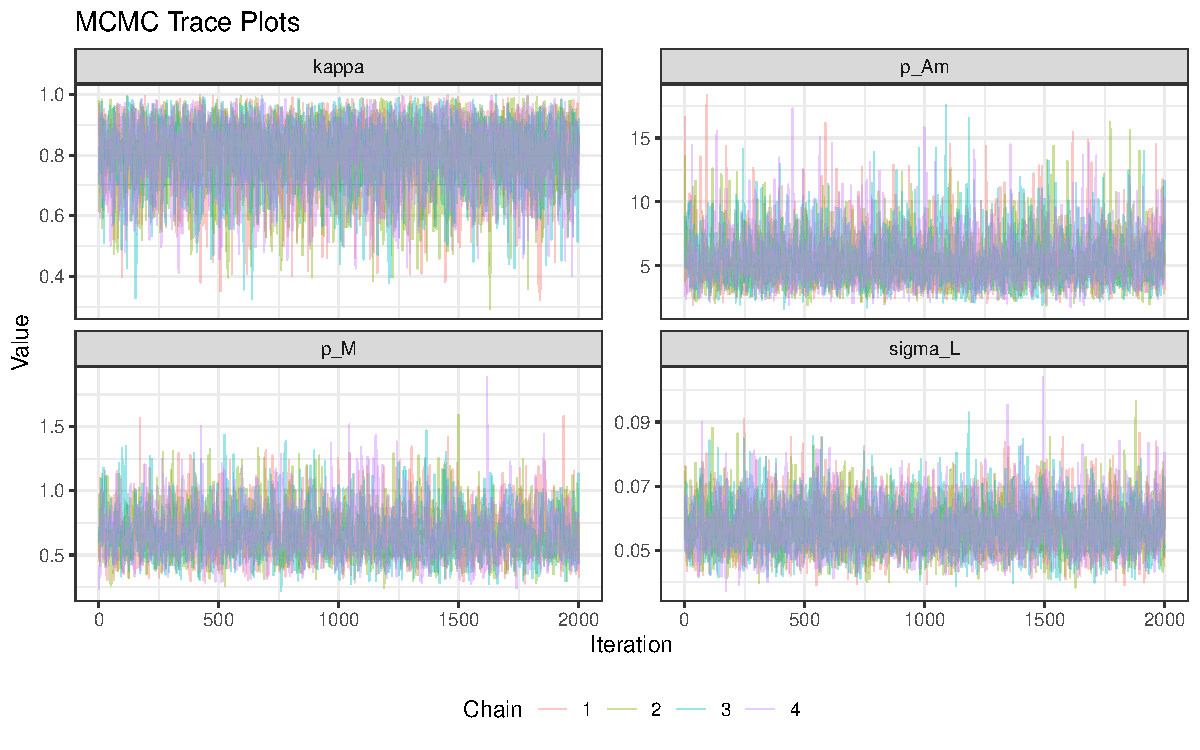
\includegraphics[width=0.8\textwidth]{fig_trace.pdf}
\caption{MCMC trace plots for core parameters ($\pAm$, $\pM$,
  $\kappa$, $\sigma_L$) from the Neuhauser (1980) fit.  All four
  chains mix well ($\hat{R} < 1.01$).}
\label{fig:diagnostics}
\end{figure}

\begin{figure}[t!]
\centering
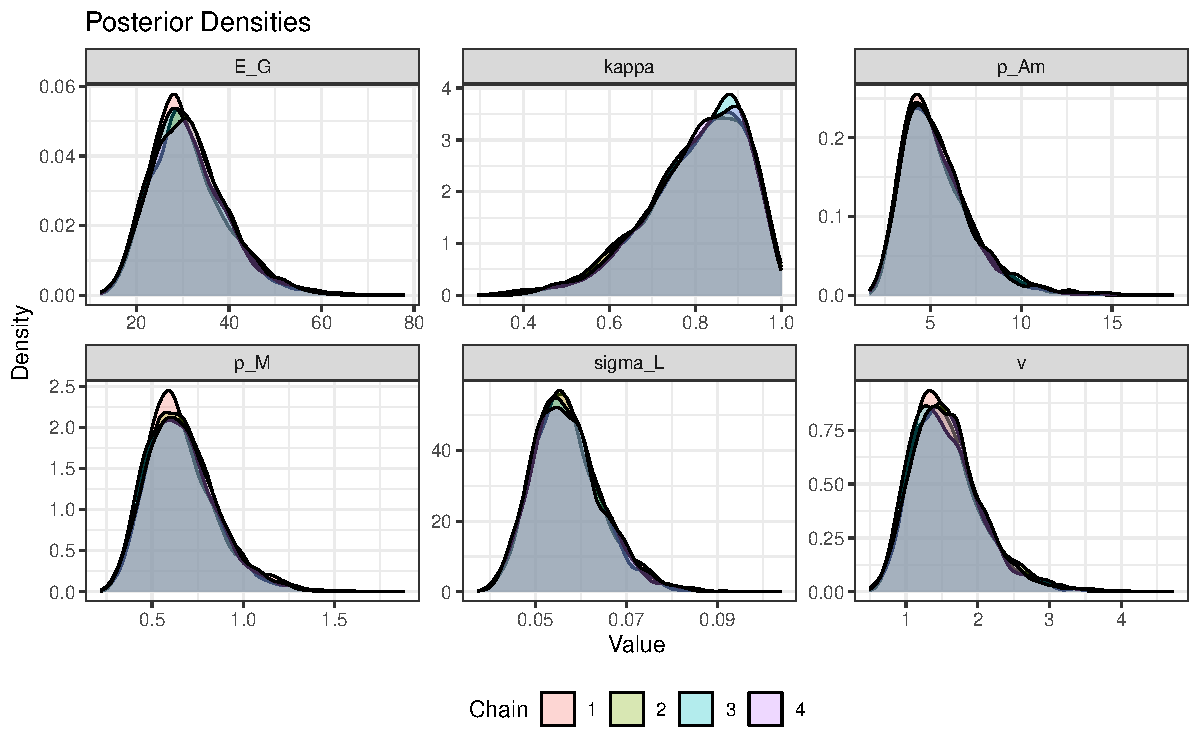
\includegraphics[width=0.8\textwidth]{fig_posterior.pdf}
\caption{Marginal posterior densities for all six DEB parameters,
  coloured by chain.  The overlap between chains confirms
  convergence.}
\label{fig:posterior}
\end{figure}

\begin{itemize}
  \item \textbf{Trace plots} (\code{type = "trace"}):
    MCMC chains over iterations for visual convergence assessment.
    Well-mixed chains appear as overlapping ``hairy caterpillars.''
  \item \textbf{Posterior densities} (\code{type = "posterior"}):
    Marginal density curves overlaid by chain, highlighting
    multi-modality or chain disagreement.
  \item \textbf{Pairs plots} (\code{type = "pairs"}):
    Bivariate posterior scatter plots revealing correlations.  The
    $\pM$--$v$ and $\pM$--$\EG$ correlations are typically the
    strongest (Section~\ref{sec:identifiability}).
  \item \textbf{Trajectory plots} (\code{type = "trajectory"}):
    Posterior predicted growth curves (blue) overlaid on observed data
    (black points), propagating parameter uncertainty.
  \item \textbf{PPC plots} (\code{plot(bdeb\_ppc(fit))}):
    Replicated data (grey) vs.\ observed data (red), assessing
    model adequacy \citep[Ch.~6]{GelmanBDA2013}.
  \item \textbf{Dose-response} (\code{plot\_dose\_response()}):
    Full-model predicted relative growth across concentrations with
    posterior uncertainty bands, EC$_{50}$ and NEC marked.
  \item \textbf{Prior vs.\ posterior} (\code{type = "prior\_posterior"}):
    Overlaid prior (red) and posterior (blue) densities for each
    parameter.  This directly visualises the contraction
    (Section~\ref{sec:identifiability}): parameters where red and
    blue overlap are prior-dominated; parameters where the posterior
    is much narrower are data-informed.
\end{itemize}

Figure~\ref{fig:prior_post} shows the prior--posterior comparison
for the Neuhauser (1980) fit.  The plot confirms the contraction
analysis: $\sigma_L$ is sharply data-determined, $\kappa$ shows
moderate updating, while $\pAm$, $\pM$, $v$, and $\EG$ remain
largely prior-shaped.

\begin{figure}[t!]
\centering
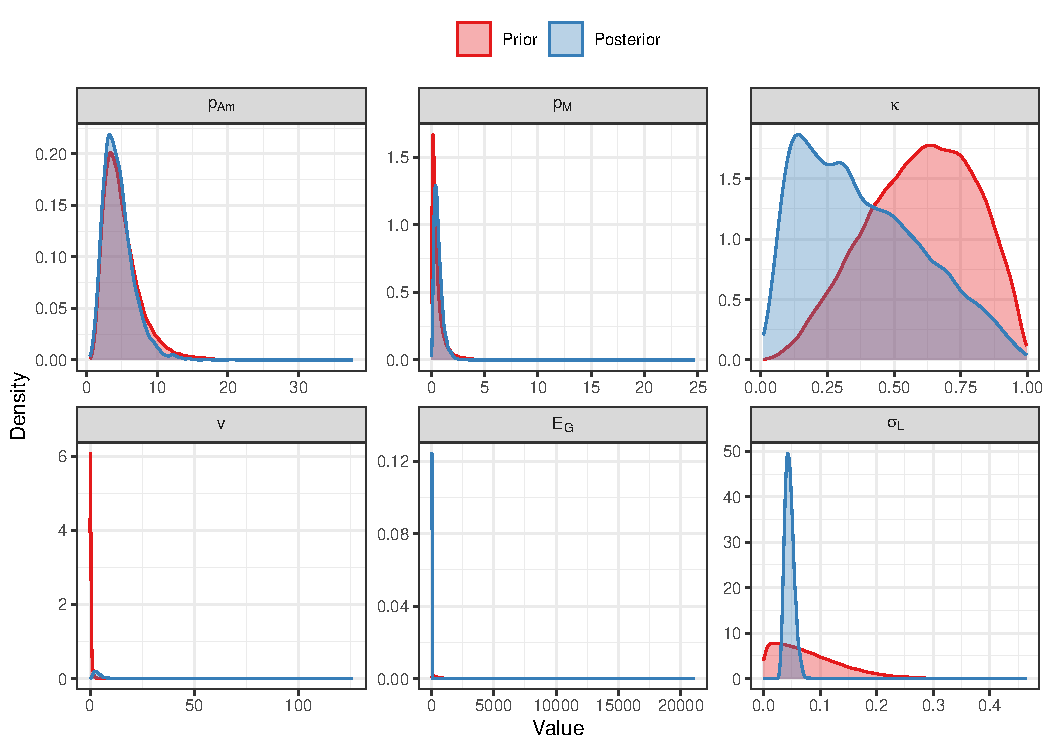
\includegraphics[width=0.85\textwidth]{fig_prior_posterior.pdf}
\caption{Prior (red) vs.\ posterior (blue) densities for six DEB
  parameters from the Neuhauser (1980) fit.  Only $\sigma_L$ and
  $\kappa$ show substantial contraction; the rate parameters
  $\pAm$, $\pM$, $v$, and $\EG$ are largely prior-driven,
  consistent with Table~\ref{tab:contraction}.}
\label{fig:prior_post}
\end{figure}

Figure~\ref{fig:prior_pred} shows a prior predictive check.

\begin{figure}[t!]
\centering
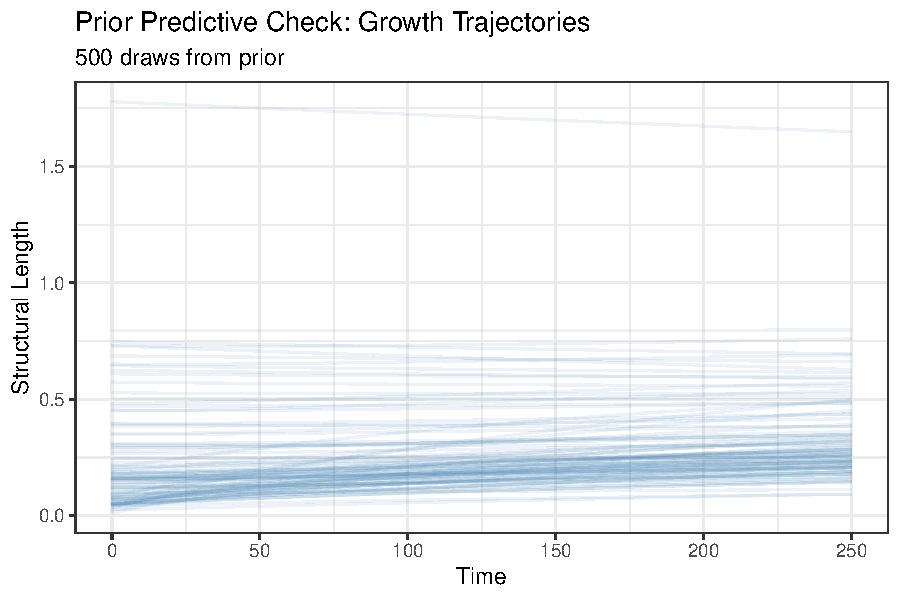
\includegraphics[width=0.8\textwidth]{fig_prior_predictive.pdf}
\caption{Prior predictive check: 500~growth trajectories sampled
  from the prior.  The spread shows the range of data the model
  considers plausible \emph{before} seeing data.}
\label{fig:prior_pred}
\end{figure}

\subsection{Computational performance} \label{sec:cost}

Table~\ref{tab:runtime} reports wall-clock times on a 16-core
workstation (AMD Ryzen 9, 64~GB RAM, Ubuntu 22.04, CmdStan~2.36.0).
Compilation is a one-time cost cached by \pkg{cmdstanr}; sampling
times are for 4~chains $\times$ 2000~iterations.

\begin{table}[t!]
\centering
\caption{Wall-clock times (seconds).  Threading shows
  parallel\_chains~$\times$~threads/chain.}
\label{tab:runtime}
\begin{tabular}{lrrrrr}
\toprule
Model & Data size & Compile & Sample & Threading & Speedup \\
\midrule
Individual     & 1 ind., 13 obs.    & 30 & 69   & $4 \times 1$ & --- \\
Individual     & 1 ind., 37 obs.    & -- & 392  & $4 \times 1$ & --- \\
Hierarchical   & 21 ind., 273 obs.  & 35 & $\sim$3200 & $4 \times 1$ & $1\times$ \\
Hierarchical   & 21 ind., 273 obs.  & -- & $\sim$900  & $2 \times 4$ & $3.6\times$ \\
DEBtox         & 4 grp., 280 obs.   & 35 & $\sim$600  & $2 \times 2$ & --- \\
\bottomrule
\end{tabular}
\end{table}

% Timings from AMD Ryzen 9, CmdStan 2.36.0, 4 chains x 2000 iter.

\paragraph{Threading speedup.}
Table~\ref{tab:runtime} shows the hierarchical model under two
threading configurations.  With $2 \times 4$ (2~parallel chains,
4~threads each, 8~cores total), wall-clock time is $3.6\times$
shorter than the sequential baseline ($4 \times 1$, 4~parallel
chains, 1~thread each).  Note that the two configurations use
different total core counts (8 vs.\ 4), so this figure reflects
both within-chain parallelism via \code{reduce\_sum} and the
change in parallel-chain scheduling; it is not a pure threading
benchmark.  The within-chain speedup arises because
\code{reduce\_sum} distributes the 21~per-individual ODE solves
across threads within each chain.

\paragraph{Scaling with dataset size.}
Sampling time scales approximately linearly with the number of
individuals in the hierarchical model, as each individual contributes
an independent ODE solve distributed via \code{reduce\_sum}.

\paragraph{Memory usage.}
Memory consumption scales linearly with $N_{\mathrm{ind}} \times
N_{\mathrm{obs}} \times N_{\mathrm{states}}$.  For the bundled
datasets, peak RSS was $<$500~MB per chain.  The dominant memory cost
is the ODE solver's internal state, not the \proglang{Stan} parameter
vector.


%% ======================================================================
\section{Comparison with existing software} \label{sec:comparison}
%% ======================================================================

\begin{table}[t!]
\centering
\caption{Comparison of \pkg{BayesianDEB} with existing DEB calibration
  tools.}
\label{tab:comparison}
\begin{tabular}{lcccc}
\toprule
Feature & AmP/\pkg{DEBtool} & \pkg{deBInfer} & Custom \proglang{Stan}
  & \pkg{BayesianDEB} \\
\midrule
Bayesian inference        & ---       & Yes & Yes & Yes \\
Pre-built DEB models      & Yes       & --- & --- & Yes \\
Hierarchical models       & ---       & --- & Manual & Built-in \\
DEBtox (TKTD)             & Partial   & --- & Manual & Built-in \\
Observation model choice  & ---       & --- & Manual & Switchable \\
Prior specification API   & ---       & Basic & Manual & 6 families \\
Temperature correction    & Manual    & --- & Manual & Built-in \\
Convergence diagnostics   & Minimal   & Basic & Manual & Automated \\
PPC                       & ---       & --- & Manual & Built-in \\
LOO-CV                    & ---       & --- & Manual & Built-in \\
Within-chain parallelism  & ---       & --- & Manual & \code{reduce\_sum} \\
\proglang{R} package      & \proglang{MATLAB}+\proglang{R} & Yes & --- & Yes \\
\bottomrule
\end{tabular}
\end{table}

Table~\ref{tab:comparison} summarises the feature landscape.
\pkg{DEBtool\_M} and the AmP estimation tool \citep{MarquesAmP2018}
are the standard DEB calibration platforms but are primarily
\proglang{MATLAB}-based, use deterministic optimisation, and do not support
hierarchical models or formal uncertainty quantification.
\pkg{deBInfer} \citep{deBInfer2017} provides Bayesian ODE inference in
\proglang{R} but requires the user to write the ODE system and does
not include DEB-specific models, ecotoxicological extensions, or
\proglang{Stan}-based samplers.  Custom \proglang{Stan} code can
implement any of these models but requires significant expertise and
has no reusable API.  \pkg{BayesianDEB} combines the model coverage of
AmP/\pkg{DEBtool} with the Bayesian inference capabilities of
\proglang{Stan}, wrapped in a user-friendly \proglang{R} interface.


%% ======================================================================
\section{Current limitations and future work} \label{sec:limitations}
%% ======================================================================

\begin{itemize}
  \item The \code{"individual"} and \code{"growth\_repro"} models
    support exactly one individual; multi-individual data require
    \code{"hierarchical"}.
  \item The \code{"debtox"} model fits one ODE per concentration group
    (group-level); individual-level hierarchical DEBtox is planned.
  \item The hierarchical model places random effects on $\pAm$ only.
  \item Temperature correction is global (single $T$ per experiment);
    time-varying temperature is planned.
  \item The survival endpoint is not yet implemented.
  \item All lengths are structural ($L = V^{1/3}$); the shape
    coefficient $\delta_M$ is not estimated.
  \item R-side simulators (\code{deb\_simulate},
    \code{bdeb\_prior\_predictive}, trajectory plots) use the LSODA
    solver from \pkg{deSolve}, which automatically switches between
    stiff (BDF) and non-stiff (Adams) methods.  For the mildly stiff
    DEB system, LSODA predominantly selects BDF steps, matching the
    fixed-BDF solver in \proglang{Stan}; numerical agreement was
    verified to $< 10^{-5}$~cm across 100~random parameter draws
    (Section~\ref{sec:sbc}).
  \item Strong posterior correlations between $\pM$, $v$, and $\EG$
    (and between $\pAm$ and $\EG$) are inherent to the DEB
    $\kappa$-rule structure (Section~\ref{sec:identifiability}).
    Informative priors are recommended.
  \item Comprehensive SBC validation (Section~\ref{sec:sbc}) has
    been performed for the individual growth model (397~valid
    replications).  Preliminary SBC for the hierarchical model
    (38~valid replications) provides encouraging but statistically
    limited evidence.  The DEBtox model has not yet been validated
    via SBC; it shares the same ODE system and observation
    likelihoods as the individual model, but its toxicokinetic
    damage component ($D_w$, $z_w$, $b_w$) warrants dedicated
    validation.  Comprehensive SBC for the hierarchical and DEBtox
    models is planned for a future version.
  \item Reparametrising the \proglang{Stan} models in terms of
    derived quantities ($L_\infty$, $g$, $k_M$) rather than primary
    parameters ($\pAm$, $\pM$, $v$) could improve both sampling
    efficiency and interpretability, as these quantities are better
    identified by growth data.  This requires a Jacobian adjustment
    in \proglang{Stan} and modification of all four model programs.
  \item Multi-endpoint inference (growth $+$ reproduction $+$
    respiration simultaneously) would substantially improve
    identifiability of rate parameters that are prior-dominated
    under growth-only data (Table~\ref{tab:contraction}).  A joint
    likelihood combining Equations~\eqref{eq:obs_L}
    and~\eqref{eq:obs_R} with a respiration observation model is a
    natural extension.
\end{itemize}


%% ======================================================================
\section{Summary} \label{sec:summary}
%% ======================================================================

\pkg{BayesianDEB} provides the first general-purpose \proglang{R}
package for Bayesian Dynamic Energy Budget modelling.  By embedding
DEB ODEs within \proglang{Stan}'s HMC framework, it delivers full
posterior uncertainty propagation to all parameters and derived
quantities, principled prior incorporation from the AmP database,
hierarchical partial pooling across individuals, and ecotoxicological
EC$_{50}$/NEC estimation with posterior uncertainty.  The declarative
\proglang{R} interface requires no \proglang{Stan} programming from
the user, while the within-chain parallelism via \code{reduce\_sum}
makes hierarchical and DEBtox models tractable on modern multi-core
hardware.

Equally important, the identifiability analysis and prior sensitivity
tools make explicit a fundamental limitation that deterministic
calibration tools obscure: for growth-only data, DEB rate parameters
are largely prior-dominated, and species-specific informative priors
or hierarchical data structures are essential for quantitative
inference.  We view this transparency as a feature, not a limitation,
of the Bayesian approach.


%% ======================================================================
%% -- Computational details (unnumbered) ---------------------------------
\section*{Computational details}

The results in this paper were obtained using
\proglang{R}~4.5.2 (2025-10-31) on \code{x86\_64-pc-linux-gnu}
(Ubuntu 22.04) with the packages listed below.
\pkg{BayesianDEB}~0.1.2 is distributed under the MIT license and
available from the SCIOM r-universe at
\url{https://sciom.r-universe.dev/BayesianDEB} and from GitHub at
\url{https://github.com/sciom/BayesianDEB}.  \pkg{cmdstanr} is
available from the Stan r-universe at
\url{https://stan-dev.r-universe.dev}.

\begin{CodeChunk}
\begin{CodeInput}
R> install.packages("BayesianDEB",
+    repos = "https://sciom.r-universe.dev")
R> install.packages("cmdstanr",
+    repos = "https://stan-dev.r-universe.dev")
R> cmdstanr::install_cmdstan()
\end{CodeInput}
\end{CodeChunk}

\begin{CodeChunk}
\begin{CodeOutput}
R version 4.5.2 (2025-10-31), x86_64-pc-linux-gnu

Attached packages:
  BayesianDEB 0.1.2, posterior 1.6.1, bayesplot 1.14.0,
  ggplot2 4.0.1, deSolve 1.42, loo 2.8.0

Loaded via namespace:
  cmdstanr 0.8.0 (CmdStan 2.36.0), rlang 1.1.7,
  cli 3.6.5, Rcpp 1.1.0
\end{CodeOutput}
\end{CodeChunk}


%% -- Acknowledgments (unnumbered) ---------------------------------------
\section*{Acknowledgments}

This work was supported by the Croatian Science Foundation (HRZZ)
under the project FUNECOSoil --- Functional Ecological
Characterization of Soils: The Basis for Ecotoxicological
Classification (grant no.\ IP-2022-10-7177).


%% -- Bibliography -------------------------------------------------------
\bibliography{bayesiandeb}

\end{document}
